% Default to the notebook output style

\documentclass[11pt]{article}

    \usepackage[T1]{fontenc}
    % Nicer default font (+ math font) than Computer Modern for most use cases
    \usepackage{mathpazo}
    

\usepackage{palatino} 
\usepackage{listings} %  Gives syntaxx highlighting for python code. 
\usepackage{color} % Used for syntax highlighting. 
\usepackage{textcomp} % Used for syntax highlighting. 

% This gives syntax highlighting in the python environment 
\renewcommand{\lstlistlistingname}{Code Listings} 
\renewcommand{\lstlistingname}{Code Listing} 
\definecolor{gray}{gray}{0.5} 
\definecolor{key}{rgb}{0,0.5,0} 
\definecolor{darkgreen}{rgb}{0,0.5,0} 
\lstnewenvironment{python}[1][]{ 
\lstset{ 
language=python, 
basicstyle=\ttfamily, 
otherkeywords={1, 2, 3, 4, 5, 6, 7, 8 ,9 , 0}, 
keywordstyle=\color{blue}, 
stringstyle=\color{red}, 
showstringspaces=false, 
emph={class, pass, in, for, while, if, is, elif, else, not, and, or, 
def, print, exec, break, continue, return}, 
emphstyle=\color{darkgreen}\bfseries, 
emph={[2]True, False, None, self}, 
emphstyle=[2]\color{blue}, 
emph={[3]from, import, as}, 
emphstyle=[3]\color{darkgreen}, 
upquote=true, 
morecomment=[s]{"""}{"""}, 
commentstyle=\color{gray}\slshape,#1 
}}{} 


% Inherit from the specified cell style.



% OKRUZENJA ZA TEOREME, LEME, DOKAZE...
\newtheorem{theorem}{\bf Teorema}[section]
\newtheorem{lemma}[theorem]{\bf Lema}
\newtheorem{corollary}[theorem]{\bf Posledica}
\newtheorem{definition}[theorem]{\bf Definicija}
\newtheorem{conjecture}[theorem]{\bf Hipoteza}
\newtheorem{remark}[theorem]{\bf Primedba}
\newtheorem{problem}[theorem]{\bf Problem}
\newtheorem{alg}[theorem]{\bf Algoritam}
\newtheorem{pri}{\bf Primer}
\newtheorem{tvrdjenje}{\bf Tvr\dj enje}

\newcommand{\comment}[1]{\ $[\![${\normalsize #1}$]\!]$ \ }
\newcommand{\proof}{\noindent{\bf Dokaz.\ }}
\newcommand{\qed}{\hfill $\square$ \bigskip}
\def\cp{\,\square\,}

%\def \dj  {d\kern-0.4em\char"16\kern-0.1em}
%\def \dj {\mbox{\raise0.3ex\hbox{-}\kern-0.4em D}}
\usepackage[serbian]{babel}
\renewcommand{\tablename}{Tabela}
\renewcommand{\figurename}{Slika}
\renewcommand{\refname}{Literatura}
\renewcommand{\abstractname}{Apstrakt}

    

    
    


    % Basic figure setup, for now with no caption control since it's done
    % automatically by Pandoc (which extracts ![](path) syntax from Markdown).
    \usepackage{graphicx}
    \usepackage{float}
    % We will generate all images so they have a width \maxwidth. This means
    % that they will get their normal width if they fit onto the page, but
    % are scaled down if they would overflow the margins.
    \makeatletter
    \def\maxwidth{\ifdim\Gin@nat@width>\linewidth\linewidth
    \else\Gin@nat@width\fi}
    \makeatother
   
    % Set max figure width to be 80% of text width, for now hardcoded.
    % Ensure that by default, figures have no caption (until we provide a
    % proper Figure object with a Caption API and a way to capture that
    % in the conversion process - todo).
    \usepackage{caption}
    \DeclareCaptionLabelFormat{nolabel}{}
    \captionsetup{labelformat=nolabel}

    \usepackage{adjustbox} % Used to constrain images to a maximum size 
    \usepackage{xcolor} % Allow colors to be defined
    \usepackage{enumerate} % Needed for markdown enumerations to work
    \usepackage{geometry} % Used to adjust the document margins
    \usepackage{amsmath} % Equations
    \usepackage{amssymb} % Equations
    \usepackage{textcomp} % defines textquotesingle
    % Hack from http://tex.stackexchange.com/a/47451/13684:
    \AtBeginDocument{%
        \def\PYZsq{\textquotesingle}% Upright quotes in Pygmentized code
    }
    \usepackage{upquote} % Upright quotes for verbatim code
    \usepackage{eurosym} % defines \euro
    \usepackage[mathletters]{ucs} % Extended unicode (utf-8) support
    \usepackage[utf8x]{inputenc} % Allow utf-8 characters in the tex document
    \usepackage{fancyvrb} % verbatim replacement that allows latex
    \usepackage{grffile} % extends the file name processing of package graphics 
                         % to support a larger range 
    % The hyperref package gives us a pdf with properly built
    % internal navigation ('pdf bookmarks' for the table of contents,
    % internal cross-reference links, web links for URLs, etc.)
    \usepackage{hyperref}
    \usepackage{longtable} % longtable support required by pandoc >1.10
    \usepackage{booktabs}  % table support for pandoc > 1.12.2
    \usepackage[inline]{enumitem} % IRkernel/repr support (it uses the enumerate* environment)
    \usepackage[normalem]{ulem} % ulem is needed to support strikethroughs (\sout)
                                % normalem makes italics be italics, not underlines
    
	\usepackage{caption}
	\usepackage{subcaption}
    \usepackage{booktabs}
    \usepackage{xcolor}
	
    % Colors for the hyperref package
    \definecolor{urlcolor}{rgb}{0,.145,.698}
    \definecolor{linkcolor}{rgb}{.71,0.21,0.01}
    \definecolor{citecolor}{rgb}{.12,.54,.11}

    % ANSI colors
    \definecolor{ansi-black}{HTML}{3E424D}
    \definecolor{ansi-black-intense}{HTML}{282C36}
    \definecolor{ansi-red}{HTML}{E75C58}
    \definecolor{ansi-red-intense}{HTML}{B22B31}
    \definecolor{ansi-green}{HTML}{00A250}
    \definecolor{ansi-green-intense}{HTML}{007427}
    \definecolor{ansi-yellow}{HTML}{DDB62B}
    \definecolor{ansi-yellow-intense}{HTML}{B27D12}
    \definecolor{ansi-blue}{HTML}{208FFB}
    \definecolor{ansi-blue-intense}{HTML}{0065CA}
    \definecolor{ansi-magenta}{HTML}{D160C4}
    \definecolor{ansi-magenta-intense}{HTML}{A03196}
    \definecolor{ansi-cyan}{HTML}{60C6C8}
    \definecolor{ansi-cyan-intense}{HTML}{258F8F}
    \definecolor{ansi-white}{HTML}{C5C1B4}
    \definecolor{ansi-white-intense}{HTML}{A1A6B2}

    % commands and environments needed by pandoc snippets
    % extracted from the output of `pandoc -s`
    \providecommand{\tightlist}{%
      \setlength{\itemsep}{0pt}\setlength{\parskip}{0pt}}
    \DefineVerbatimEnvironment{Highlighting}{Verbatim}{commandchars=\\\{\}}
    % Add ',fontsize=\small' for more characters per line
    \newenvironment{Shaded}{}{}
    \newcommand{\KeywordTok}[1]{\textcolor[rgb]{0.00,0.44,0.13}{\textbf{{#1}}}}
    \newcommand{\DataTypeTok}[1]{\textcolor[rgb]{0.56,0.13,0.00}{{#1}}}
    \newcommand{\DecValTok}[1]{\textcolor[rgb]{0.25,0.63,0.44}{{#1}}}
    \newcommand{\BaseNTok}[1]{\textcolor[rgb]{0.25,0.63,0.44}{{#1}}}
    \newcommand{\FloatTok}[1]{\textcolor[rgb]{0.25,0.63,0.44}{{#1}}}
    \newcommand{\CharTok}[1]{\textcolor[rgb]{0.25,0.44,0.63}{{#1}}}
    \newcommand{\StringTok}[1]{\textcolor[rgb]{0.25,0.44,0.63}{{#1}}}
    \newcommand{\CommentTok}[1]{\textcolor[rgb]{0.38,0.63,0.69}{\textit{{#1}}}}
    \newcommand{\OtherTok}[1]{\textcolor[rgb]{0.00,0.44,0.13}{{#1}}}
    \newcommand{\AlertTok}[1]{\textcolor[rgb]{1.00,0.00,0.00}{\textbf{{#1}}}}
    \newcommand{\FunctionTok}[1]{\textcolor[rgb]{0.02,0.16,0.49}{{#1}}}
    \newcommand{\RegionMarkerTok}[1]{{#1}}
    \newcommand{\ErrorTok}[1]{\textcolor[rgb]{1.00,0.00,0.00}{\textbf{{#1}}}}
    \newcommand{\NormalTok}[1]{{#1}}
    
    % Additional commands for more recent versions of Pandoc
    \newcommand{\ConstantTok}[1]{\textcolor[rgb]{0.53,0.00,0.00}{{#1}}}
    \newcommand{\SpecialCharTok}[1]{\textcolor[rgb]{0.25,0.44,0.63}{{#1}}}
    \newcommand{\VerbatimStringTok}[1]{\textcolor[rgb]{0.25,0.44,0.63}{{#1}}}
    \newcommand{\SpecialStringTok}[1]{\textcolor[rgb]{0.73,0.40,0.53}{{#1}}}
    \newcommand{\ImportTok}[1]{{#1}}
    \newcommand{\DocumentationTok}[1]{\textcolor[rgb]{0.73,0.13,0.13}{\textit{{#1}}}}
    \newcommand{\AnnotationTok}[1]{\textcolor[rgb]{0.38,0.63,0.69}{\textbf{\textit{{#1}}}}}
    \newcommand{\CommentVarTok}[1]{\textcolor[rgb]{0.38,0.63,0.69}{\textbf{\textit{{#1}}}}}
    \newcommand{\VariableTok}[1]{\textcolor[rgb]{0.10,0.09,0.49}{{#1}}}
    \newcommand{\ControlFlowTok}[1]{\textcolor[rgb]{0.00,0.44,0.13}{\textbf{{#1}}}}
    \newcommand{\OperatorTok}[1]{\textcolor[rgb]{0.40,0.40,0.40}{{#1}}}
    \newcommand{\BuiltInTok}[1]{{#1}}
    \newcommand{\ExtensionTok}[1]{{#1}}
    \newcommand{\PreprocessorTok}[1]{\textcolor[rgb]{0.74,0.48,0.00}{{#1}}}
    \newcommand{\AttributeTok}[1]{\textcolor[rgb]{0.49,0.56,0.16}{{#1}}}
    \newcommand{\InformationTok}[1]{\textcolor[rgb]{0.38,0.63,0.69}{\textbf{\textit{{#1}}}}}
    \newcommand{\WarningTok}[1]{\textcolor[rgb]{0.38,0.63,0.69}{\textbf{\textit{{#1}}}}}
    
    
    % Define a nice break command that doesn't care if a line doesn't already
    % exist.
    \def\br{\hspace*{\fill} \\* }
    % Math Jax compatability definitions
	\def\TeX{\mbox{T\kern-.14em\lower.5ex\hbox{E}\kern-.115em X}}
	\def\LaTeX{\mbox{L\kern-.325em\raise.21em\hbox{$\scriptstyle{A}$}\kern-.17em}\TeX}

    \def\gt{>}
    \def\lt{<}
    % Document parameters
    \title{Kristalografske grupe i poplo\v cavanje}
    \author{
Marina Vasiljevi\' c \\
Matemati\v cka gimnazija \\
e-mail: \tt{marina.vasiljevic@petlja.org} \\
\\
 }
    
    

    % Pygments definitions
    
\makeatletter
\def\PY@reset{\let\PY@it=\relax \let\PY@bf=\relax%
    \let\PY@ul=\relax \let\PY@tc=\relax%
    \let\PY@bc=\relax \let\PY@ff=\relax}
\def\PY@tok#1{\csname PY@tok@#1\endcsname}
\def\PY@toks#1+{\ifx\relax#1\empty\else%
    \PY@tok{#1}\expandafter\PY@toks\fi}
\def\PY@do#1{\PY@bc{\PY@tc{\PY@ul{%
    \PY@it{\PY@bf{\PY@ff{#1}}}}}}}
\def\PY#1#2{\PY@reset\PY@toks#1+\relax+\PY@do{#2}}

\expandafter\def\csname PY@tok@gd\endcsname{\def\PY@tc##1{\textcolor[rgb]{0.63,0.00,0.00}{##1}}}
\expandafter\def\csname PY@tok@gu\endcsname{\let\PY@bf=\textbf\def\PY@tc##1{\textcolor[rgb]{0.50,0.00,0.50}{##1}}}
\expandafter\def\csname PY@tok@gt\endcsname{\def\PY@tc##1{\textcolor[rgb]{0.00,0.27,0.87}{##1}}}
\expandafter\def\csname PY@tok@gs\endcsname{\let\PY@bf=\textbf}
\expandafter\def\csname PY@tok@gr\endcsname{\def\PY@tc##1{\textcolor[rgb]{1.00,0.00,0.00}{##1}}}
\expandafter\def\csname PY@tok@cm\endcsname{\let\PY@it=\textit\def\PY@tc##1{\textcolor[rgb]{0.25,0.50,0.50}{##1}}}
\expandafter\def\csname PY@tok@vg\endcsname{\def\PY@tc##1{\textcolor[rgb]{0.10,0.09,0.49}{##1}}}
\expandafter\def\csname PY@tok@vi\endcsname{\def\PY@tc##1{\textcolor[rgb]{0.10,0.09,0.49}{##1}}}
\expandafter\def\csname PY@tok@vm\endcsname{\def\PY@tc##1{\textcolor[rgb]{0.10,0.09,0.49}{##1}}}
\expandafter\def\csname PY@tok@mh\endcsname{\def\PY@tc##1{\textcolor[rgb]{0.40,0.40,0.40}{##1}}}
\expandafter\def\csname PY@tok@cs\endcsname{\let\PY@it=\textit\def\PY@tc##1{\textcolor[rgb]{0.25,0.50,0.50}{##1}}}
\expandafter\def\csname PY@tok@ge\endcsname{\let\PY@it=\textit}
\expandafter\def\csname PY@tok@vc\endcsname{\def\PY@tc##1{\textcolor[rgb]{0.10,0.09,0.49}{##1}}}
\expandafter\def\csname PY@tok@il\endcsname{\def\PY@tc##1{\textcolor[rgb]{0.40,0.40,0.40}{##1}}}
\expandafter\def\csname PY@tok@go\endcsname{\def\PY@tc##1{\textcolor[rgb]{0.53,0.53,0.53}{##1}}}
\expandafter\def\csname PY@tok@cp\endcsname{\def\PY@tc##1{\textcolor[rgb]{0.74,0.48,0.00}{##1}}}
\expandafter\def\csname PY@tok@gi\endcsname{\def\PY@tc##1{\textcolor[rgb]{0.00,0.63,0.00}{##1}}}
\expandafter\def\csname PY@tok@gh\endcsname{\let\PY@bf=\textbf\def\PY@tc##1{\textcolor[rgb]{0.00,0.00,0.50}{##1}}}
\expandafter\def\csname PY@tok@ni\endcsname{\let\PY@bf=\textbf\def\PY@tc##1{\textcolor[rgb]{0.60,0.60,0.60}{##1}}}
\expandafter\def\csname PY@tok@nl\endcsname{\def\PY@tc##1{\textcolor[rgb]{0.63,0.63,0.00}{##1}}}
\expandafter\def\csname PY@tok@nn\endcsname{\let\PY@bf=\textbf\def\PY@tc##1{\textcolor[rgb]{0.00,0.00,1.00}{##1}}}
\expandafter\def\csname PY@tok@no\endcsname{\def\PY@tc##1{\textcolor[rgb]{0.53,0.00,0.00}{##1}}}
\expandafter\def\csname PY@tok@na\endcsname{\def\PY@tc##1{\textcolor[rgb]{0.49,0.56,0.16}{##1}}}
\expandafter\def\csname PY@tok@nb\endcsname{\def\PY@tc##1{\textcolor[rgb]{0.00,0.50,0.00}{##1}}}
\expandafter\def\csname PY@tok@nc\endcsname{\let\PY@bf=\textbf\def\PY@tc##1{\textcolor[rgb]{0.00,0.00,1.00}{##1}}}
\expandafter\def\csname PY@tok@nd\endcsname{\def\PY@tc##1{\textcolor[rgb]{0.67,0.13,1.00}{##1}}}
\expandafter\def\csname PY@tok@ne\endcsname{\let\PY@bf=\textbf\def\PY@tc##1{\textcolor[rgb]{0.82,0.25,0.23}{##1}}}
\expandafter\def\csname PY@tok@nf\endcsname{\def\PY@tc##1{\textcolor[rgb]{0.00,0.00,1.00}{##1}}}
\expandafter\def\csname PY@tok@si\endcsname{\let\PY@bf=\textbf\def\PY@tc##1{\textcolor[rgb]{0.73,0.40,0.53}{##1}}}
\expandafter\def\csname PY@tok@s2\endcsname{\def\PY@tc##1{\textcolor[rgb]{0.73,0.13,0.13}{##1}}}
\expandafter\def\csname PY@tok@nt\endcsname{\let\PY@bf=\textbf\def\PY@tc##1{\textcolor[rgb]{0.00,0.50,0.00}{##1}}}
\expandafter\def\csname PY@tok@nv\endcsname{\def\PY@tc##1{\textcolor[rgb]{0.10,0.09,0.49}{##1}}}
\expandafter\def\csname PY@tok@s1\endcsname{\def\PY@tc##1{\textcolor[rgb]{0.73,0.13,0.13}{##1}}}
\expandafter\def\csname PY@tok@dl\endcsname{\def\PY@tc##1{\textcolor[rgb]{0.73,0.13,0.13}{##1}}}
\expandafter\def\csname PY@tok@ch\endcsname{\let\PY@it=\textit\def\PY@tc##1{\textcolor[rgb]{0.25,0.50,0.50}{##1}}}
\expandafter\def\csname PY@tok@m\endcsname{\def\PY@tc##1{\textcolor[rgb]{0.40,0.40,0.40}{##1}}}
\expandafter\def\csname PY@tok@gp\endcsname{\let\PY@bf=\textbf\def\PY@tc##1{\textcolor[rgb]{0.00,0.00,0.50}{##1}}}
\expandafter\def\csname PY@tok@sh\endcsname{\def\PY@tc##1{\textcolor[rgb]{0.73,0.13,0.13}{##1}}}
\expandafter\def\csname PY@tok@ow\endcsname{\let\PY@bf=\textbf\def\PY@tc##1{\textcolor[rgb]{0.67,0.13,1.00}{##1}}}
\expandafter\def\csname PY@tok@sx\endcsname{\def\PY@tc##1{\textcolor[rgb]{0.00,0.50,0.00}{##1}}}
\expandafter\def\csname PY@tok@bp\endcsname{\def\PY@tc##1{\textcolor[rgb]{0.00,0.50,0.00}{##1}}}
\expandafter\def\csname PY@tok@c1\endcsname{\let\PY@it=\textit\def\PY@tc##1{\textcolor[rgb]{0.25,0.50,0.50}{##1}}}
\expandafter\def\csname PY@tok@fm\endcsname{\def\PY@tc##1{\textcolor[rgb]{0.00,0.00,1.00}{##1}}}
\expandafter\def\csname PY@tok@o\endcsname{\def\PY@tc##1{\textcolor[rgb]{0.40,0.40,0.40}{##1}}}
\expandafter\def\csname PY@tok@kc\endcsname{\let\PY@bf=\textbf\def\PY@tc##1{\textcolor[rgb]{0.00,0.50,0.00}{##1}}}
\expandafter\def\csname PY@tok@c\endcsname{\let\PY@it=\textit\def\PY@tc##1{\textcolor[rgb]{0.25,0.50,0.50}{##1}}}
\expandafter\def\csname PY@tok@mf\endcsname{\def\PY@tc##1{\textcolor[rgb]{0.40,0.40,0.40}{##1}}}
\expandafter\def\csname PY@tok@err\endcsname{\def\PY@bc##1{\setlength{\fboxsep}{0pt}\fcolorbox[rgb]{1.00,0.00,0.00}{1,1,1}{\strut ##1}}}
\expandafter\def\csname PY@tok@mb\endcsname{\def\PY@tc##1{\textcolor[rgb]{0.40,0.40,0.40}{##1}}}
\expandafter\def\csname PY@tok@ss\endcsname{\def\PY@tc##1{\textcolor[rgb]{0.10,0.09,0.49}{##1}}}
\expandafter\def\csname PY@tok@sr\endcsname{\def\PY@tc##1{\textcolor[rgb]{0.73,0.40,0.53}{##1}}}
\expandafter\def\csname PY@tok@mo\endcsname{\def\PY@tc##1{\textcolor[rgb]{0.40,0.40,0.40}{##1}}}
\expandafter\def\csname PY@tok@kd\endcsname{\let\PY@bf=\textbf\def\PY@tc##1{\textcolor[rgb]{0.00,0.50,0.00}{##1}}}
\expandafter\def\csname PY@tok@mi\endcsname{\def\PY@tc##1{\textcolor[rgb]{0.40,0.40,0.40}{##1}}}
\expandafter\def\csname PY@tok@kn\endcsname{\let\PY@bf=\textbf\def\PY@tc##1{\textcolor[rgb]{0.00,0.50,0.00}{##1}}}
\expandafter\def\csname PY@tok@cpf\endcsname{\let\PY@it=\textit\def\PY@tc##1{\textcolor[rgb]{0.25,0.50,0.50}{##1}}}
\expandafter\def\csname PY@tok@kr\endcsname{\let\PY@bf=\textbf\def\PY@tc##1{\textcolor[rgb]{0.00,0.50,0.00}{##1}}}
\expandafter\def\csname PY@tok@s\endcsname{\def\PY@tc##1{\textcolor[rgb]{0.73,0.13,0.13}{##1}}}
\expandafter\def\csname PY@tok@kp\endcsname{\def\PY@tc##1{\textcolor[rgb]{0.00,0.50,0.00}{##1}}}
\expandafter\def\csname PY@tok@w\endcsname{\def\PY@tc##1{\textcolor[rgb]{0.73,0.73,0.73}{##1}}}
\expandafter\def\csname PY@tok@kt\endcsname{\def\PY@tc##1{\textcolor[rgb]{0.69,0.00,0.25}{##1}}}
\expandafter\def\csname PY@tok@sc\endcsname{\def\PY@tc##1{\textcolor[rgb]{0.73,0.13,0.13}{##1}}}
\expandafter\def\csname PY@tok@sb\endcsname{\def\PY@tc##1{\textcolor[rgb]{0.73,0.13,0.13}{##1}}}
\expandafter\def\csname PY@tok@sa\endcsname{\def\PY@tc##1{\textcolor[rgb]{0.73,0.13,0.13}{##1}}}
\expandafter\def\csname PY@tok@k\endcsname{\let\PY@bf=\textbf\def\PY@tc##1{\textcolor[rgb]{0.00,0.50,0.00}{##1}}}
\expandafter\def\csname PY@tok@se\endcsname{\let\PY@bf=\textbf\def\PY@tc##1{\textcolor[rgb]{0.73,0.40,0.13}{##1}}}
\expandafter\def\csname PY@tok@sd\endcsname{\let\PY@it=\textit\def\PY@tc##1{\textcolor[rgb]{0.73,0.13,0.13}{##1}}}

\def\PYZbs{\char`\\}
\def\PYZus{\char`\_}
\def\PYZob{\char`\{}
\def\PYZcb{\char`\}}
\def\PYZca{\char`\^}
\def\PYZam{\char`\&}
\def\PYZlt{\char`\<}
\def\PYZgt{\char`\>}
\def\PYZsh{\char`\#}
\def\PYZpc{\char`\%}
\def\PYZdl{\char`\$}
\def\PYZhy{\char`\-}
\def\PYZsq{\char`\'}
\def\PYZdq{\char`\"}
\def\PYZti{\char`\~}
% for compatibility with earlier versions
\def\PYZat{@}
\def\PYZlb{[}
\def\PYZrb{]}
\makeatother


    % Exact colors from NB
    \definecolor{incolor}{rgb}{0.0, 0.0, 0.5}
    \definecolor{outcolor}{rgb}{0.545, 0.0, 0.0}



    
    % Prevent overflowing lines due to hard-to-break entities
    \sloppy 
    % Setup hyperref package
    \hypersetup{
      breaklinks=true,  % so long urls are correctly broken across lines
      colorlinks=true,
      urlcolor=urlcolor,
      linkcolor=linkcolor,https://v1.overleaf.com/dash
      citecolor=citecolor,
      }
    % Slightly bigger margins than the latex defaults
    
    \geometry{verbose,tmargin=1in,bmargin=1in,lmargin=1in,rmargin=1in}
    
    

\begin{document} 
    
    \maketitle
    
    
\begin{abstract}
U radu se bavimo konstruisanjem fundamentalnih oblasti za kristalografske grupe euklidske ravni. Matemati\v cki je opisana metoda konstrukcije zasnovana na uop\v stenju Dirihleovog domena i implementirana je ra\v cunarska aplikacija koja efektivno konstrui\v se fundamentalne domene kori\v scenjem te metode. Korisnik aplikacije klikom mi\v sa ucrtava ta\v cke. Na osnovu zadatih ta\v caka program konsturi\v se fundamentalni domen kome pripradaju sve ta\v cke ravni koje su bli\v ze nekoj od zadatih ta\v caka nego nekoj od njihovih slika u izometrijama iz kristalografske grupe i u realnom vremenu se iscrtava dobijeno poplo\v cavanje. Aplikacija ima opciju da izabrani skup ta\v caka posmatra kao temena poligonalne linije, na osnovu koje se konstrui\v se fundamentalni domen kao skup ta\v caka ravni kojima je ta poligonalna linija bli\v za neko bilo koja njena slika. Tako dobijen fundamentalni domen je vi\v se gladak. 
\end{abstract}

\section{Uvod}\label{kristalografske-grupe-i-poploux10davanje}

Popločavanje je prekrivanje ravni ili prostora geometrijskim figurama čije se unutrašnjosti ne preklapaju. Takve figure nazivamo pločicama ili teselima od latinske reči tessella koja označava parče kamena ili stakla od koga se slaže mozaik. Posebno
su zanimljiva popločavanja kod kojih se koriste podudarne firgure tako
da imamo grupu izometrija koje jednu figuru preslikavaju na sve ostale.
Jedan od primera takvog popločavanja su kristalne rešetke, zbog čega se
takve grupe nazivaju kristalografskim grupama.

U ovom radu ćemo se baviti popločavanjima u euklidskoj ravni
\(\mathbb{E}^2\). Prvo ćemo definisati pojam kristalografske grupe u
\(\mathbb{E}^2\).

\begin{definition} Za grupu \(G\) kažemo da je konačno
generisana ako postoji konačan podskup elemenata grupe koji generiše sve
elemente grupe
\end{definition}

\begin{definition} Konačna fundamentalna oblast \(F\)
grupe izometrija \(G\) u \(\mathbb{E}^2\) je unija konačno mnogo
poligona takva da važi:\\
\begin{enumerate}
\item \(\displaystyle{\bigcup_{g\in G}g(F)} = \mathbb{E}^2\) 
\item \((\forall g\in G)(\mathring{F} \cap g(\mathring{F})= \emptyset)\)
\end{enumerate}
\end{definition}
    Fundamentalna oblasta po definiciji u opštem slučaju ne mora da bude
poligon ali je za potrebe ovog rada dovoljno da se ograničimo na
poligone. Takođe, opštija definicija bi zahtevala pojmove iz topologije,
dok smo se ovako zadržali da geometrijskoj terminologiji.

\begin{definition} Kristalografska grupa je konačno
generisana grupa izometrija koja ima konačnu fundamentalnu oblast.
\end{definition}
    Poznato je da u \(\mathbb{E}^2\) postoji 17 različitih (do na
izomorfizam) kristalografskih grupa. Ovde mislimo na algebarski
izomorfizam grupa.

    U okviru ovog rada bavićemo se svojstvima kristalografskih grupa u
\(\mathbb{E}^2\), svojstvima fundamentalnih oblasti i algoritmima za
konstruisanje fundamentalnih poligona koji na kraju mogu imati praktičnu
primenu u grafičkom dizajniranju popločavanja. Algoritme ćemo
implementirati u programskom jeziku Python.

    \section{\texorpdfstring{Izometrijske transformacije u
\(\mathbb{R}^2\)}{Izometrijske transformacije u \textbackslash{}mathbb\{R\}\^{}2}}\label{izometrijske-transformacije-u-mathbbr2}

    Ako u \(\mathbb{E}^2\) uvedemo koordinatni sistem, tačke predstavljamo
dvodimenzionim koordinatama tj. elementima \(\mathbb{R}^2\). Koordinate
tacke \(A\) označavaćemo sa \((A_x, A_y)\). Analitički ćemo izometrijsku
transformaciju u \(\mathbb{R}^2\) predstaviti kao specijalan slučaj
afine transformacije. Ako je \(A' = g(A)\) tada imamo:
\[A'_x = pA_x + qA_y + c_x\] \[A'_y = rA_x + sA_y + c_y\] Korišćenjem
računa sa matricama to možemo predstaviti:

\[\begin{bmatrix}p & q\\ r & s\end{bmatrix} \begin{bmatrix}A_x\\ A_y \end{bmatrix} + \begin{bmatrix}c_x\\ c_y\end{bmatrix} = \begin{bmatrix}A'_x\\ A'_y \end{bmatrix}\]

Korišćenjem homogenih koordinata ovo možemo predstaviti kao množenje
trodimenzionih matrica:

\[\begin{bmatrix}p & q & c_x\\ r & s&c_y \\ 0 & 0 & 1\end{bmatrix} \begin{bmatrix}A_x\\ A_y\\1\end{bmatrix} = 
\begin{bmatrix}A'_x\\ A'_y\\1\end{bmatrix}\]

Na primer, translacija za vektor \((t_x, t_y)\) bi se predstavila kao:

\[\begin{bmatrix}1 & 0 & t_x\\ 0 & 1&t_y \\ 0 & 0 & 1\end{bmatrix} \begin{bmatrix}A_x\\ A_y\\1\end{bmatrix} = 
\begin{bmatrix}A_x+t_x\\ A_y+t_y\\1\end{bmatrix}\]

\begin{pri}Primer sa konkretnim brojevima u sintaksi programskog jezika Python:
\end{pri}  

\begin{python}
tx,ty = 5,6
t = np.array([
    [ 1,  0,  tx],
    [ 0,  1,  ty],
    [ 0,  0,  1] ])
A = np.array([2,3,1])
t @ A
\end{python} 

    U primeru smo translirali tačku \(A(2,3)\) za vektor \((5,6)\), što daje rezultat:
    
\begin{python}
array([7, 9, 1])
\end{python}

    \subsection{Funkcije koje konstruišu matrice za osnovne izomejtrijske
transformacije}\label{funkcije-koje-konstruiux161u-matrice-za-osnovne-izomejtrijske-transformacije}

    Funkcija \texttt{transl} konstruiše matricu za translaciju:

\begin{python}
def transl(tx,ty):
    return np.array([
        [ 1,  0,  tx],
        [ 0,  1,  ty],
        [ 0,  0,  1]])
\end{python}


    Funkcija \texttt{rot0} konstruiše matricu za rotaciju oko koordinatnog
početka za zadati ugao:

\begin{Verbatim}[commandchars=\\\{\}]
\PY{k}{def} \PY{n+nf}{rot0}\PY{p}{(}\PY{n}{fi}\PY{p}{)}\PY{p}{:}
    \PY{k}{return} \PY{n}{np}\PY{o}{.}\PY{n}{array}\PY{p}{(}\PY{p}{[}
        \PY{p}{[} \PY{n}{cos}\PY{p}{(}\PY{n}{fi}\PY{p}{)}\PY{p}{,}  \PY{n}{sin}\PY{p}{(}\PY{n}{fi}\PY{p}{)}\PY{p}{,}  \PY{l+m+mi}{0}\PY{p}{]}\PY{p}{,}
        \PY{p}{[}\PY{o}{\PYZhy{}}\PY{n}{sin}\PY{p}{(}\PY{n}{fi}\PY{p}{)}\PY{p}{,}  \PY{n}{cos}\PY{p}{(}\PY{n}{fi}\PY{p}{)}\PY{p}{,}  \PY{l+m+mi}{0}\PY{p}{]}\PY{p}{,}
        \PY{p}{[}       \PY{l+m+mi}{0}\PY{p}{,}        \PY{l+m+mi}{0}\PY{p}{,}    \PY{l+m+mi}{1}\PY{p}{]} \PY{p}{]}\PY{p}{)}
\end{Verbatim}


    Funkcija \texttt{reflX} konstruiše matricu za refleksiju oko x-ose:

    \begin{Verbatim}[commandchars=\\\{\}]
\PY{k}{def} \PY{n+nf}{reflX}\PY{p}{(}\PY{p}{)}\PY{p}{:}
    \PY{k}{return} \PY{n}{np}\PY{o}{.}\PY{n}{array}\PY{p}{(}\PY{p}{[}
        \PY{p}{[} \PY{l+m+mi}{1}\PY{p}{,}   \PY{l+m+mi}{0}\PY{p}{,}  \PY{l+m+mi}{0}\PY{p}{]}\PY{p}{,}
        \PY{p}{[} \PY{l+m+mi}{0}\PY{p}{,}  \PY{o}{\PYZhy{}}\PY{l+m+mi}{1}\PY{p}{,}  \PY{l+m+mi}{0}\PY{p}{]}\PY{p}{,}
        \PY{p}{[} \PY{l+m+mi}{0}\PY{p}{,}   \PY{l+m+mi}{0}\PY{p}{,}  \PY{l+m+mi}{1}\PY{p}{]} \PY{p}{]}\PY{p}{)}
\end{Verbatim}


    Prednost korišćenja homogenih koordinata je u tome što slaganje
izometrija računamo kao množenje matrica. Na taj način funkciju
\texttt{rot}, koja konstruiše matricu za rotaciju oko zadate tačke,
možemo definisati kao:

    \begin{Verbatim}[commandchars=\\\{\}]
\PY{k}{def} \PY{n+nf}{rot}\PY{p}{(}\PY{n}{fi}\PY{p}{,} \PY{n}{cx}\PY{p}{,} \PY{n}{cy}\PY{p}{)} \PY{n} \\
   \PY{k}{return} \PY{n}{transl}\PY{p}{(}\PY{n}{cx}\PY{p}{,} \PY{n}{cy}\PY{p}{)} \PY{o}{@}  \PY{n}{rot0}\PY{p}{(}\PY{n}{fi}\PY{p}{)} \PY{o}{@} \PY{n}{transl}\PY{p}{(}\PY{o}{\PYZhy{}}\PY{n}{cx}\PY{p}{,} \PY{o}{\PYZhy{}} \PY{n}{cy}\PY{p}{)}
    
   \end{Verbatim}
Specijalno, centralnu simetriju defini\v semo kao rotaciju za ugao $\pi$ :
\begin{Verbatim}[commandchars=\\\{\}]
\PY{k}{def} \PY{n+nf}{sim0}\PY{p}{(}\PY{n}{cx} \PY{p}{,}\PY{n}{cy}\PY{p}{)}\PY{p}{:}
    \PY{k}{return} \PY{n}{rot}\PY{p}{(}\PY{n}{pi}\PY{p}{,}\PY{n}{cx}\PY{p}{,}\PY{n}{cy}\PY{p}{)}
\end{Verbatim}


    Slično konstruišemo refleksiju oko proizvoljne ose zadate koordinatama
jedne tačke na toj osi i uglom koji ona pravi sa x-osom:

    \begin{Verbatim}[commandchars=\\\{\}]
\PY{k}{def} \PY{n+nf}{refl}\PY{p}{(}\PY{n}{ax}\PY{p}{,}\PY{n}{ay}\PY{p}{,}\PY{n}{fi}\PY{p}{)}\PY{p}{:}
    \PY{k}{return} \PY{n}{transl}\PY{p}{(}\PY{n}{ax}\PY{p}{,}\PY{n}{ay}\PY{p}{)} \PY{o}{@} \PY{n}{rot0}\PY{p}{(}\PY{n}{fi}\PY{p}{)} \PY{o}{@} \PY{n}{reflX}\PY{p}{(}\PY{p}{)} \PY{o}{@} \PY{n}{rot0}\PY{p}{(}\PY{o}{\PYZhy{}}\PY{n}{fi}\PY{p}{)} \PY{o}{@} \PY{n}{transl}\PY{p}{(}\PY{o}{\PYZhy{}}\PY{n}{ax}\PY{p}{,}\PY{o}{\PYZhy{}}\PY{n}{ay}\PY{p}{)}
\end{Verbatim}


    Ukoliko osa prolazi kroz koordinatni početak i tačku $a$, matricu osne
refleksije možemo i direktno konstruisati bez primene trigonometrijskih
funkcija na sledeći način:

    \begin{Verbatim}[commandchars=\\\{\}]
\PY{k}{def} \PY{n+nf}{refl1}\PY{p}{(}\PY{n}{ax}\PY{p}{,}\PY{n}{ay}\PY{p}{)}\PY{p}{:}
    \PY{n}{r} \PY{o}{=} \PY{p}{(}\PY{n}{ax}\PY{o}{*}\PY{n}{ax}\PY{o}{+}\PY{n}{ay}\PY{o}{*}\PY{n}{ay}\PY{p}{)} 
    \PY{k}{return} \PY{n}{np}\PY{o}{.}\PY{n}{array}\PY{p}{(}\PY{p}{[}
        \PY{p}{[} \PY{p}{(}\PY{n}{ax}\PY{o}{*}\PY{n}{ax}\PY{o}{\PYZhy{}}\PY{n}{ay}\PY{o}{*}\PY{n}{ay}\PY{p}{)}\PY{o}{/}\PY{n}{r}\PY{p}{,}  \PY{l+m+mi}{2}\PY{o}{*}\PY{n}{ax}\PY{o}{*}\PY{n}{ay}\PY{o}{/}\PY{n}{r}\PY{p}{,}  \PY{l+m+mi}{0}\PY{p}{]}\PY{p}{,}
        \PY{p}{[} \PY{l+m+mi}{2}\PY{o}{*}\PY{n}{ax}\PY{o}{*}\PY{n}{ay}\PY{o}{/}\PY{n}{r}\PY{p}{,} \PY{p}{(}\PY{n}{ay}\PY{o}{*}\PY{n}{ay}\PY{o}{\PYZhy{}}\PY{n}{ax}\PY{o}{*}\PY{n}{ax}\PY{p}{)}\PY{o}{/}\PY{n}{r} \PY{p}{,}  \PY{l+m+mi}{0}\PY{p}{]}\PY{p}{,}
        \PY{p}{[}         \PY{l+m+mi}{0}\PY{p}{,}                \PY{l+m+mi}{0}\PY{p}{,}  \PY{l+m+mi}{1}\PY{p}{]} \PY{p}{]}\PY{p}{)}
\end{Verbatim}


    Koristeći to možemo konstruisati refleksiju oko ose zadate dvema tačkama

    \begin{Verbatim}[commandchars=\\\{\}]
\PY{k}{def} \PY{n+nf}{refl2}\PY{p}{(}\PY{n}{ax}\PY{p}{,}\PY{n}{ay}\PY{p}{,}\PY{n}{bx}\PY{p}{,}\PY{n}{by}\PY{p}{)}\PY{p}{:}
    \PY{k}{return} \PY{n}{transl}\PY{p}{(}\PY{n}{ax}\PY{p}{,}\PY{n}{ay}\PY{p}{)}\PY{n+nd}{@refl1}\PY{p}{(}\PY{n}{bx}\PY{o}{\PYZhy{}}\PY{n}{ax}\PY{p}{,}\PY{n}{by}\PY{o}{\PYZhy{}}\PY{n}{ay}\PY{p}{)}\PY{n+nd}{@transl}\PY{p}{(}\PY{o}{\PYZhy{}}\PY{n}{ax}\PY{p}{,}\PY{o}{\PYZhy{}}\PY{n}{ay}\PY{p}{)}
\end{Verbatim}


    Klizajuću refleksiju predstavljamo kao kompoziciju translacije i
refleksije

    \begin{Verbatim}[commandchars=\\\{\}]
\PY{k}{def} \PY{n+nf}{glref}\PY{p}{(}\PY{n}{ax}\PY{p}{,}\PY{n}{ay}\PY{p}{,}\PY{n}{bx}\PY{p}{,}\PY{n}{by}\PY{p}{)}\PY{p}{:}
    \PY{k}{return} \PY{n}{refl2}\PY{p}{(}\PY{n}{ax}\PY{p}{,}\PY{n}{ay}\PY{p}{,}\PY{n}{bx}\PY{p}{,}\PY{n}{by}\PY{p}{)}\PY{n+nd}{@transl}\PY{p}{(}\PY{p}{(}\PY{n}{bx}\PY{o}{\PYZhy{}}\PY{n}{ax}\PY{p}{)}\PY{p}{,}\PY{p}{(}\PY{n}{by}\PY{o}{\PYZhy{}}\PY{n}{ay}\PY{p}{)}\PY{p}{)}
\end{Verbatim}


    \subsection{Predstavljanje grupa homogenim matricama i njihova
implementacija}\label{predstavljanje-grupa-homogenim-matricama-i-njihova-implementacija}
Pri konstruisanju svake grupe koristi\' cemo jedini\v cnu matricu i inverz matrice koje defini\v semo redom kao:

\begin{Verbatim}[commandchars=\\\{\}]
\PY{n}{I} \PY{o}{=} \PY{n}{np}\PY{o}{.}\PY{n}{array}\PY{p}{(}\PY{p}{[}
    \PY{p}{[} \PY{l+m+mi}{1}\PY{p}{,}  \PY{l+m+mi}{0}\PY{p}{,}  \PY{l+m+mi}{0}\PY{p}{]}\PY{p}{,}
    \PY{p}{[} \PY{l+m+mi}{0}\PY{p}{,}  \PY{l+m+mi}{1}\PY{p}{,}  \PY{l+m+mi}{0}\PY{p}{]}\PY{p}{,}
    \PY{p}{[} \PY{l+m+mi}{0}\PY{p}{,}  \PY{l+m+mi}{0}\PY{p}{,}  \PY{l+m+mi}{1}\PY{p}{]}\PY{p}{]}\PY{p}{)}
\PY{k}{def} \PY{n+nf}{inv}\PY{p}{(}\PY{n}{x}\PY{p}{)}\PY{p}{:}
    \PY{k}{return} \PY{n}{np}\PY{o}{.}\PY{n}{linalg}\PY{o}{.}\PY{n}{inv}\PY{p}{(}\PY{n}{x}\PY{p}{)}
\end{Verbatim}

    Grupu \textbf{p1} generišu dve translacije. Ako vektore te dve translacije označimo sa u i v, odgovarajuće homogene matrice su:

\[\begin{bmatrix}1 & 0 & v_x\\ 0 & 1&v_y \\ 0 & 0 & 1\end{bmatrix}, \begin{bmatrix}1 & 0 & u_x\\ 0 & 1&u_y \\ 0 & 0 & 1\end{bmatrix}\]

Koristićemo skup generatora grupe koji je proširen inverznim  izometrijama i identitetom,  pa je implementacija grupe \textbf{p1} sa parametrima:

    


    \begin{Verbatim}[commandchars=\\\{\}]
\PY{k}{def} \PY{n+nf}{p1}\PY{p}{(}\PY{n}{ux}\PY{p}{,}\PY{n}{uy}\PY{p}{,}\PY{n}{vx}\PY{p}{,}\PY{n}{vy}\PY{p}{)}\PY{p}{:}
    \PY{n}{tr_u} \PY{o}{=} \PY{n}{transl}\PY{p}{(}\PY{n}{ux}\PY{p}{,} \PY{n}{uy}\PY{p}{)}
    \PY{n}{tr_v} \PY{o}{=} \PY{n}{transl}\PY{p}{(}\PY{n}{vx}\PY{p}{,} \PY{n}{vy}\PY{p}{)}
    \PY{k}{return} \PY{p}{[}\PY{n}{I}\PY{p}{,}\PY{n}{tr_u}\PY{p}{,}\PY{n}{tr_v}\PY{p}{,}\PY{n}{inv}\PY{p}{(}\PY{n}{tr_u}\PY{p}{)}\PY{p}{,} \PY{n}{inv}\PY{p}{(}\PY{n}{tr_v}\PY{p}{)}\PY{p}{]}
\end{Verbatim}


    Grupu \textbf{p2} generi\v su tri centralne simetrije. Fundamentalni domen može
biti trougaoni ili četvorougaoni. Radi lakšeg implementiranja, kao generatore \' cemo posmatrati jednu simetriju (kojom fundamentalni domen proširujemo
do paralelograma) i dve translacije. Generi\v semo ga pomo\' cu vektora tih
translacija i koordinata jedne fiksne ta\v cke.

\[\begin{Bmatrix}\begin{bmatrix}-1 & 0 & 2a_x +v_x+u_x\\ 0 & -1& 2a_y +v_y+u_y \\ 0 & 0 & 1\end{bmatrix}&,& \begin{bmatrix}1 & 0 & v_x\\ 0 & 1&v_y \\ 0 & 0 & 1\end{bmatrix}&,& \begin{bmatrix}1 & 0 & u_x\\ 0 & 1&u_y \\ 0 & 0 & 1\end{bmatrix}  \end{Bmatrix}\]

    \begin{Verbatim}[commandchars=\\\{\}]
\PY{k}{def} \PY{n+nf}{p2}\PY{p}{(}\PY{n}{ax}\PY{p}{,}\PY{n}{ay}\PY{p}{,}\PY{n}{x1}\PY{p}{,}\PY{n}{y1}\PY{p}{,}\PY{n}{x2}\PY{p}{,}\PY{n}{y2}\PY{p}{)}\PY{p}{:}
    \PY{n}{sym} \PY{o}{=} \PY{n}{rot}\PY{p}{(}\PY{n}{pi}\PY{p}{,}\PY{n}{ax}\PY{p}{,}\PY{n}{ay}\PY{p}{)}
    \PY{k}{return} \PY{n}{p1}\PY{p}{(}\PY{l+m+mi}{2}\PY{o}{*}\PY{n}{x1}\PY{p}{,}\PY{l+m+mi}{2}\PY{o}{*}\PY{n}{x2}\PY{p}{,}\PY{n}{y1}\PY{p}{,}\PY{n}{y2}\PY{p}{)} \PY{o}{+} \PY{p}{[}\PY{n}{sym}\PY{p}{,} \PY{n}{inv}\PY{p}{(}\PY{n}{sym}\PY{p}{)}\PY{p}{]}
\end{Verbatim}


    Grupu \textbf{pm} generi\v su refleksije i translacije. Podrazumevani fundamentalni domen je
pravougaonik . U programu ga generi\v semo preko koordinata jednog temena i dva vektora.

\[\begin{Bmatrix}\begin{bmatrix} \frac{v_{x}^{2}-v_{y}^{2} }{v_{x}^{2}+v_{y}^{2}}& \frac{2v_{x}v_{y}}{v_{x}^{2}+v_{y}^{2}}& \frac{2a_yv_{x}v_{y} + a_x(v_{x}^{2}-v_{y}^{2}-1)}{v_{x}^{2}+v_{y}^{2}}\\\frac{2v_{x}v_{y}}{v_{x}^{2}+v_{y}^{2}}&\frac{v_{y}^{2}-v_{x}^{2} }{v_{x}^{2}+v_{y}^{2}}& \frac{2a_xv_{x}v_{y} + a_y(v_{x}^{2}-v_{y}^{2}-1)}{v_{x}^{2}+v_{y}^{2}} \\ 0 & 0 & 1\end{bmatrix} & ,& \begin{bmatrix}1 & 0 & 2v_x\\ 0 & 1&2v_y \\ 0 & 0 & 1\end{bmatrix}& ,& \begin{bmatrix}1 & 0 & u_x\\ 0 & 1&u_y \\ 0 & 0 & 1\end{bmatrix}  \end{Bmatrix}\]

    \begin{Verbatim}[commandchars=\\\{\}]
\PY{k}{def} \PY{n+nf}{pm}\PY{p}{(}\PY{n}{ax}\PY{p}{,}\PY{n}{ay}\PY{p}{,}\PY{n}{x1}\PY{p}{,}\PY{n}{y1}\PY{p}{,}\PY{n}{x2}\PY{p}{,}\PY{n}{y2}\PY{p}{)}\PY{p}{:}
    \PY{n}{ref} \PY{o}{=} \PY{n}{refl2}\PY{p}{(}\PY{n}{ax}\PY{p}{,}\PY{n}{ay}\PY{p}{,} \PY{n}{ax}\PY{o}{+}\PY{n}{x1}\PY{p}{,}\PY{n}{ay}\PY{o}{+}\PY{n}{y1}\PY{p}{)}
    \PY{k}{return} \PY{n}{p1}\PY{p}{(}\PY{n}{x1}\PY{p}{,}\PY{n}{y1}\PY{p}{,}\PY{l+m+mi}{2}\PY{o}{*}\PY{n}{x2}\PY{p}{,}\PY{l+m+mi}{2}\PY{o}{*}\PY{n}{y2}\PY{p}{)} \PY{o}{+}\PY{p}{[}\PY{n}{ref}\PY{p}{]}
\end{Verbatim}

    Grupu \textbf{pmm} generi\v su dve refleksije i translacije, fundamentalni domen je pravougaonik.
    
    \begin{Verbatim}[commandchars=\\\{\}]
\PY{k}{def} \PY{n+nf}{pmm}\PY{p}{(}\PY{n}{ax}\PY{p}{,}\PY{n}{ay}\PY{p}{,} \PY{n}{x1}\PY{p}{,}\PY{n}{y1}\PY{p}{,}\PY{n}{x2}\PY{p}{,}\PY{n}{y2}\PY{p}{)}\PY{p}{:}
    \PY{n}{ref1} \PY{o}{=} \PY{n}{refl2}\PY{p}{(}\PY{n}{ax}\PY{p}{,}\PY{n}{ay}\PY{p}{,} \PY{n}{ax}\PY{o}{+}\PY{n}{x1}\PY{p}{,} \PY{n}{ay}\PY{o}{+}\PY{n}{y1}\PY{p}{)}
    \PY{n}{ref2} \PY{o}{=} \PY{n}{refl2}\PY{p}{(}\PY{n}{ax}\PY{p}{,}\PY{n}{ay}\PY{p}{,} \PY{n}{ax}\PY{o}{+}\PY{n}{x2}\PY{p}{,} \PY{n}{ay}\PY{o}{+}\PY{n}{y2}\PY{p}{)}
    \PY{k}{return} \PY{p}{[}\PY{n}{ref1}\PY{p}{,}\PY{n}{ref2}\PY{p}{]} \PY{o}{+} \PY{n}{p1}\PY{p}{(}\PY{l+m+mi}{2}\PY{o}{*}\PY{n}{x1}\PY{p}{,}\PY{l+m+mi}{2}\PY{o}{*}\PY{n}{y1}\PY{p}{,} \PY{l+m+mi}{2}\PY{o}{*}\PY{n}{x2}\PY{p}{,}\PY{l+m+mi}{2}\PY{o}{*}\PY{n}{y2}\PY{p}{)}
\end{Verbatim}


    Grupu \textbf{pg} generi\v su klizaju\' ca refleksija, refleksija i translacija.

    \begin{Verbatim}[commandchars=\\\{\}]
\PY{k}{def} \PY{n+nf}{pg}\PY{p}{(}\PY{n}{ax}\PY{p}{,}\PY{n}{ay}\PY{p}{,}\PY{n}{x1}\PY{p}{,}\PY{n}{y1}\PY{p}{,}\PY{n}{x2}\PY{p}{,}\PY{n}{y2}\PY{p}{)}\PY{p}{:}
    \PY{n}{ref} \PY{o}{=} \PY{n}{refl2}\PY{p}{(}\PY{n}{ax}\PY{p}{,}\PY{n}{ay}\PY{p}{,} \PY{n}{ax}\PY{o}{+}\PY{n}{x1}\PY{p}{,} \PY{n}{ay}\PY{o}{+}\PY{n}{y1}\PY{p}{)}
    \PY{n}{gler} \PY{o}{=} \PY{n}{glref}\PY{p}{(}\PY{n}{ax} \PY{o}{+} \PY{n}{x2}\PY{o}{/}\PY{l+m+mi}{2}\PY{p}{,} \PY{n}{ay} \PY{o}{+} \PY{n}{y2}\PY{o}{/}\PY{l+m+mi}{2}\PY{p}{,} \PY{n}{ax} \PY{o}{+} \PY{n}{x1} \PY{o}{+} \PY{n}{x2}\PY{o}{/}\PY{l+m+mi}{2}\PY{p}{,} \PY{n}{ay} \PY{o}{+} \PY{n}{y1} \PY{o}{+} \PY{n}{y2}\PY{o}{/}\PY{l+m+mi}{2}\PY{p}{)}
    \PY{n}{trans} \PY{o}{=} \PY{n}{transl}\PY{p}{(}\PY{o}{\PYZhy{}}\PY{l+m+mi}{2}\PY{o}{*}\PY{n}{x1}\PY{p}{,}\PY{o}{\PYZhy{}}\PY{l+m+mi}{2}\PY{o}{*}\PY{n}{y1}\PY{p}{)}
    \PY{k}{return} \PY{p}{[}\PY{n}{I}\PY{p}{,}\PY{n}{ref}\PY{p}{,}\PY{n}{gler}\PY{p}{,} \PY{n}{trans}\PY{p}{]}
\end{Verbatim}


    Grupu \textbf{cm} generi\v su refleksije i klizaju\'ca refleksija. 
    \begin{Verbatim}[commandchars=\\\{\}]
\PY{k}{def} \PY{n+nf}{cm}\PY{p}{(}\PY{n}{ax}\PY{p}{,}\PY{n}{ay}\PY{p}{,}\PY{n}{bx}\PY{p}{,}\PY{n}{by}\PY{p}{,}\PY{n}{cx}\PY{p}{,}\PY{n}{cy}\PY{p}{)}\PY{p}{:} 
    \PY{n}{glref1} \PY{o}{=} \PY{n}{glref}\PY{p}{(}\PY{p}{(}\PY{n}{ax}\PY{o}{+}\PY{n}{cx}\PY{p}{)}\PY{o}{/}\PY{l+m+mi}{2}\PY{p}{,}\PY{p}{(}\PY{n}{ay}\PY{o}{+}\PY{n}{cy}\PY{p}{)}\PY{o}{/}\PY{l+m+mi}{2}\PY{p}{,} \PY{p}{(}\PY{n}{bx}\PY{o}{+}\PY{n}{cx}\PY{p}{)}\PY{o}{/}\PY{l+m+mi}{2}\PY{p}{,}\PY{p}{(}\PY{n}{by}\PY{o}{+}\PY{n}{cy}\PY{p}{)}\PY{o}{/}\PY{l+m+mi}{2}\PY{p}{)}
    \PY{n}{ref2} \PY{o}{=} \PY{n}{refl2}\PY{p}{(}\PY{n}{ax}\PY{p}{,}\PY{n}{ay}\PY{p}{,}\PY{n}{bx}\PY{p}{,}\PY{n}{by}\PY{p}{)}
    \PY{k}{return} \PY{p}{[}\PY{n}{I}\PY{p}{,}\PY{n}{ref2}\PY{p}{,}\PY{n}{glref1}\PY{p}{,} \PY{n}{inv}\PY{p}{(}\PY{n}{glref1}\PY{p}{)}\PY{p}{]}
\end{Verbatim}


    Grupu \textbf{p3} generi\v su tri rotacije za ugao \(\frac{2\pi}{3}\) oko temena jednakostrani\v cnog trougla.

    \begin{Verbatim}[commandchars=\\\{\}]
\PY{k}{def} \PY{n+nf}{p3}\PY{p}{(}\PY{n}{ax}\PY{p}{,}\PY{n}{ay}\PY{p}{,}\PY{n}{bx}\PY{p}{,}\PY{n}{by}\PY{p}{,}\PY{n}{cx}\PY{p}{,}\PY{n}{cy}\PY{p}{)}\PY{p}{:} 
    \PY{n}{r1} \PY{o}{=} \PY{n}{rot}\PY{p}{(}\PY{l+m+mi}{2}\PY{o}{*}\PY{n}{pi}\PY{o}{/}\PY{l+m+mi}{3}\PY{p}{,} \PY{n}{ax}\PY{p}{,}\PY{n}{ay}\PY{p}{)}
    \PY{n}{r2} \PY{o}{=} \PY{n}{rot}\PY{p}{(}\PY{l+m+mi}{2}\PY{o}{*}\PY{n}{pi}\PY{o}{/}\PY{l+m+mi}{3}\PY{p}{,}\PY{n}{bx}\PY{p}{,}\PY{n}{by}\PY{p}{)}
    \PY{n}{r3} \PY{o}{=} \PY{n}{rot}\PY{p}{(}\PY{l+m+mi}{2}\PY{o}{*}\PY{n}{pi}\PY{o}{/}\PY{l+m+mi}{3}\PY{p}{,}\PY{n}{cx}\PY{p}{,}\PY{n}{cy}\PY{p}{)}
    \PY{k}{return} \PY{p}{[}\PY{n}{I}\PY{p}{,} \PY{n}{r1}\PY{p}{,}\PY{n}{r2}\PY{p}{,}\PY{n}{r3}\PY{p}{]}
\end{Verbatim}

\begin{samepage}
    Grupu \textbf{p3m1} generu\v su rotacije za ugao \(\frac{2\pi}{3}\) oko temena jednakostrani\v cnog trougla i refleksije preko stranica tog trougla.
    \begin{Verbatim}[commandchars=\\\{\}]
\PY{k}{def} \PY{n+nf}{p3m1}\PY{p}{(}\PY{n}{ax}\PY{p}{,}\PY{n}{ay}\PY{p}{,}\PY{n}{bx}\PY{p}{,}\PY{n}{by}\PY{p}{,}\PY{n}{cx}\PY{p}{,}\PY{n}{cy}\PY{p}{)}\PY{p}{:} 
    \PY{n}{r1} \PY{o}{=} \PY{n}{rot}\PY{p}{(}\PY{l+m+mi}{2}\PY{o}{*}\PY{n}{pi}\PY{o}{/}\PY{l+m+mi}{3}\PY{p}{,} \PY{n}{ax}\PY{p}{,}\PY{n}{ay}\PY{p}{)}
    \PY{n}{r2} \PY{o}{=} \PY{n}{rot}\PY{p}{(}\PY{l+m+mi}{2}\PY{o}{*}\PY{n}{pi}\PY{o}{/}\PY{l+m+mi}{3}\PY{p}{,}\PY{n}{bx}\PY{p}{,}\PY{n}{by}\PY{p}{)}
    \PY{n}{r3} \PY{o}{=} \PY{n}{rot}\PY{p}{(}\PY{l+m+mi}{2}\PY{o}{*}\PY{n}{pi}\PY{o}{/}\PY{l+m+mi}{3}\PY{p}{,}\PY{n}{cx}\PY{p}{,}\PY{n}{cy}\PY{p}{)}
    \PY{n}{ref} \PY{o}{=} \PY{n}{refl2}\PY{p}{(}\PY{n}{ax}\PY{p}{,}\PY{n}{ay}\PY{p}{,}\PY{n}{bx}\PY{p}{,}\PY{n}{by}\PY{p}{)}
    \PY{k}{return} \PY{p}{[}\PY{n}{I}\PY{p}{,} \PY{n}{ref}\PY{p}{,}\PY{n}{r1}\PY{p}{,}\PY{n}{r2}\PY{p}{,}\PY{n}{r3}\PY{p}{]}
\end{Verbatim}
\end{samepage}

    Grupu \textbf{p31m} generi\v su rotacije za ugao \(\frac{2\pi}{3}\) oko svih
temena i refleksiju preko osnovice trougla sa uglovima \(\frac{2\pi}{3}\), \(\frac{\pi}{6}\), \(\frac{\pi}{6}\) (tre\' cina jednakostrani\v cnog trougla).

    \begin{Verbatim}[commandchars=\\\{\}]
\PY{k}{def} \PY{n+nf}{p31m}\PY{p}{(}\PY{n}{ax}\PY{p}{,}\PY{n}{ay}\PY{p}{,}\PY{n}{bx}\PY{p}{,}\PY{n}{by}\PY{p}{,}\PY{n}{cx}\PY{p}{,}\PY{n}{cy}\PY{p}{)}\PY{p}{:} 
    \PY{n}{r1} \PY{o}{=} \PY{n}{rot}\PY{p}{(}\PY{l+m+mi}{2}\PY{o}{*}\PY{n}{pi}\PY{o}{/}\PY{l+m+mi}{3}\PY{p}{,}\PY{n}{cx}\PY{p}{,}\PY{n}{cy}\PY{p}{)}
    \PY{n}{ref} \PY{o}{=} \PY{n}{refl2}\PY{p}{(}\PY{n}{ax}\PY{p}{,}\PY{n}{ay}\PY{p}{,}\PY{n}{bx}\PY{p}{,}\PY{n}{by}\PY{p}{)}
    \PY{k}{return} \PY{p}{[}\PY{n}{I}\PY{p}{,}\PY{n}{r1}\PY{p}{,}\PY{n}{ref}\PY{p}{]}
\end{Verbatim}


    Grupu \textbf{p6} generi\v su rotacije za ugao \(\frac{2\pi}{3}\) oko gornjeg temena i \(\frac{\pi}{3}\) oko temena na osnovici trougla sa uglovima \(\frac{2\pi}{3}\), \(\frac{\pi}{6}\), \(\frac{\pi}{6}\).

    \begin{Verbatim}[commandchars=\\\{\}]
\PY{k}{def} \PY{n+nf}{p6}\PY{p}{(}\PY{n}{ax}\PY{p}{,}\PY{n}{ay}\PY{p}{,}\PY{n}{bx}\PY{p}{,}\PY{n}{by}\PY{p}{,}\PY{n}{cx}\PY{p}{,}\PY{n}{cy}\PY{p}{)}\PY{p}{:} 
    \PY{n}{r1} \PY{o}{=} \PY{n}{rot}\PY{p}{(}\PY{n}{pi}\PY{o}{/}\PY{l+m+mi}{3}\PY{p}{,} \PY{n}{ax}\PY{p}{,}\PY{n}{ay}\PY{p}{)}
    \PY{n}{r2} \PY{o}{=} \PY{n}{rot}\PY{p}{(}\PY{n}{pi}\PY{o}{/}\PY{l+m+mi}{3}\PY{p}{,}\PY{n}{bx}\PY{p}{,}\PY{n}{by}\PY{p}{)}
    \PY{n}{r3} \PY{o}{=} \PY{n}{rot}\PY{p}{(}\PY{l+m+mi}{2}\PY{o}{*}\PY{n}{pi}\PY{o}{/}\PY{l+m+mi}{3}\PY{p}{,}\PY{n}{cx}\PY{p}{,}\PY{n}{cy}\PY{p}{)}
    \PY{k}{return} \PY{p}{[}\PY{n}{I}\PY{p}{,}\PY{n}{r1}\PY{p}{,}\PY{n}{r2}\PY{p}{,}\PY{n}{r3}\PY{p}{]}
\end{Verbatim}


    Grupu \textbf{p6m} generi\v su rotacije za ugao \(\frac{2\pi}{3}\) oko temena sa nepravim uglovima u pravouglom trouglu sa uglovima \(\frac{\pi}{6}\) \(\frac{\pi}{3}\) i refleksija oko kra\' ce katete.


    \begin{Verbatim}[commandchars=\\\{\}]
\PY{k}{def} \PY{n+nf}{p6m}\PY{p}{(}\PY{n}{ax}\PY{p}{,}\PY{n}{ay}\PY{p}{,}\PY{n}{bx}\PY{p}{,}\PY{n}{by}\PY{p}{,}\PY{n}{cx}\PY{p}{,}\PY{n}{cy}\PY{p}{)}\PY{p}{:} 
    \PY{n}{r1} \PY{o}{=} \PY{n}{rot}\PY{p}{(}\PY{n}{pi}\PY{o}{/}\PY{l+m+mi}{3}\PY{p}{,} \PY{n}{ax}\PY{p}{,}\PY{n}{ay}\PY{p}{)}
    \PY{n}{r2} \PY{o}{=} \PY{n}{rot}\PY{p}{(}\PY{n}{pi}\PY{o}{/}\PY{l+m+mi}{3}\PY{p}{,}\PY{l+m+mi}{2}\PY{o}{*}\PY{n}{bx}\PY{p}{,}\PY{l+m+mi}{2}\PY{o}{*}\PY{n}{by}\PY{p}{)}
    \PY{n}{ref} \PY{o}{=} \PY{n}{refl2}\PY{p}{(}\PY{n}{bx}\PY{p}{,}\PY{n}{by}\PY{p}{,}\PY{n}{cx}\PY{p}{,}\PY{n}{cy}\PY{p}{)}
    \PY{k}{return} \PY{p}{[}\PY{n}{I}\PY{p}{,}\PY{n}{r1}\PY{p}{,}\PY{n}{r2}\PY{p}{,}\PY{n}{ref}\PY{p}{]}
\end{Verbatim}


    Grupu \textbf{p4} generi\v su rotacije za ugao \(\frac{\pi}{2}\) oko dva naspramna temena kvadrata i centralna simetrija oko preostala dva.


    \begin{Verbatim}[commandchars=\\\{\}]
\PY{k}{def} \PY{n+nf}{p4}\PY{p}{(}\PY{n}{ax}\PY{p}{,}\PY{n}{ay}\PY{p}{,}\PY{n}{bx}\PY{p}{,}\PY{n}{by}\PY{p}{,}\PY{n}{cx}\PY{p}{,}\PY{n}{cy}\PY{p}{)}\PY{p}{:} 
    \PY{n}{r1} \PY{o}{=} \PY{n}{rot}\PY{p}{(}\PY{n}{pi}\PY{o}{/}\PY{l+m+mi}{2}\PY{p}{,} \PY{n}{ax}\PY{p}{,}\PY{n}{ay}\PY{p}{)}
    \PY{n}{r2} \PY{o}{=} \PY{n}{rot}\PY{p}{(}\PY{n}{pi}\PY{o}{/}\PY{l+m+mi}{2}\PY{p}{,}\PY{n}{cx}\PY{p}{,}\PY{n}{cy}\PY{p}{)}
    \PY{n}{r3} \PY{o}{=} \PY{n}{rot}\PY{p}{(}\PY{n}{pi}\PY{p}{,}\PY{n}{bx}\PY{p}{,}\PY{n}{by}\PY{p}{)}
    \PY{k}{return} \PY{p}{[}\PY{n}{I}\PY{p}{,}\PY{n}{r1}\PY{p}{,}\PY{n}{r2}\PY{p}{,}\PY{n}{r3}\PY{p}{]}
\end{Verbatim}

\begin{samepage}
    Grupa \textbf{p4m} generi\v su rotacije za ugao \(\frac{\pi}{2}\) oko dva temena na hipotenuzi, centralna simetrija oko temena pravog ugla i jedna refleksija oko hipotenuze u jednakokrako-pravouglom trouglu.

    \begin{Verbatim}[commandchars=\\\{\}]
\PY{k}{def} \PY{n+nf}{p4m}\PY{p}{(}\PY{n}{ax}\PY{p}{,}\PY{n}{ay}\PY{p}{,}\PY{n}{bx}\PY{p}{,}\PY{n}{by}\PY{p}{,}\PY{n}{cx}\PY{p}{,}\PY{n}{cy}\PY{p}{)}\PY{p}{:}
    \PY{n}{r1} \PY{o}{=} \PY{n}{rot}\PY{p}{(}\PY{n}{pi}\PY{o}{/}\PY{l+m+mi}{2}\PY{p}{,} \PY{n}{ax}\PY{p}{,}\PY{n}{ay}\PY{p}{)}
    \PY{n}{r2} \PY{o}{=} \PY{n}{rot}\PY{p}{(}\PY{n}{pi}\PY{o}{/}\PY{l+m+mi}{2}\PY{p}{,} \PY{n}{cx}\PY{p}{,}\PY{n}{cy}\PY{p}{)}
    \PY{n}{ref} \PY{o}{=} \PY{n}{refl2}\PY{p}{(}\PY{n}{bx}\PY{p}{,}\PY{n}{by}\PY{p}{,}\PY{n}{cx}\PY{p}{,}\PY{n}{cy}\PY{p}{)}
    \PY{k}{return} \PY{p}{[}\PY{n}{I}\PY{p}{,}\PY{n}{r1}\PY{p}{,}\PY{n}{r2}\PY{p}{,}\PY{n}{ref}\PY{p}{]}
\end{Verbatim}
\end{samepage}

    Grupa \textbf{cmm} generi\v su dve centralne simetrije, jedna rotacija za ugao ${\frac{\pi}{2}}$ i dve refleksije.

    \begin{Verbatim}[commandchars=\\\{\}]
\PY{k}{def} \PY{n+nf}{cmm}\PY{p}{(}\PY{n}{ax}\PY{p}{,}\PY{n}{ay}\PY{p}{,}\PY{n}{bx}\PY{p}{,}\PY{n}{by}\PY{p}{,}\PY{n}{cx}\PY{p}{,}\PY{n}{cy}\PY{p}{)}\PY{p}{:}
    \PY{n}{r1} \PY{o}{=} \PY{n}{rot}\PY{p}{(}\PY{n}{pi}\PY{p}{,} \PY{n}{ax}\PY{p}{,}\PY{n}{ay}\PY{p}{)}
    \PY{n}{r2} \PY{o}{=} \PY{n}{rot}\PY{p}{(}\PY{n}{pi}\PY{o}{/}\PY{l+m+mi}{2}\PY{p}{,} \PY{n}{bx}\PY{p}{,}\PY{n}{by}\PY{p}{)}
    \PY{n}{r3} \PY{o}{=} \PY{n}{rot}\PY{p}{(}\PY{n}{pi}\PY{p}{,}\PY{p}{(}\PY{n}{ax}\PY{o}{+}\PY{n}{cx}\PY{p}{)}\PY{o}{/}\PY{l+m+mi}{2}\PY{p}{,}\PY{p}{(}\PY{n}{ay}\PY{o}{+}\PY{n}{cy}\PY{p}{)}\PY{o}{/}\PY{l+m+mi}{2} \PY{p}{)}
    \PY{n}{ref} \PY{o}{=} \PY{n}{refl2}\PY{p}{(}\PY{n}{bx}\PY{p}{,}\PY{n}{by}\PY{p}{,}\PY{n}{cx}\PY{p}{,}\PY{n}{cy}\PY{p}{)}
    \PY{n}{ref2} \PY{o}{=} \PY{n}{refl2}\PY{p}{(}\PY{n}{ax}\PY{p}{,}\PY{n}{ay}\PY{p}{,}\PY{n}{bx}\PY{p}{,}\PY{n}{by}\PY{p}{)}
    \PY{k}{return} \PY{p}{[}\PY{n}{I}\PY{p}{,}\PY{n}{r1}\PY{p}{,}\PY{n}{r2}\PY{p}{,}\PY{n}{r3}\PY{p}{]}
\end{Verbatim}


    Grupa \textbf{p4g} generi\v su centralna simetrija, refleksija i rotacija za ugao ${\frac{\pi}{2}}$

    \begin{Verbatim}[commandchars=\\\{\}]
\PY{k}{def} \PY{n+nf}{p4g}\PY{p}{(}\PY{n}{ax}\PY{p}{,}\PY{n}{ay}\PY{p}{,}\PY{n}{bx}\PY{p}{,}\PY{n}{by}\PY{p}{,}\PY{n}{cx}\PY{p}{,}\PY{n}{cy}\PY{p}{)}\PY{p}{:}
    \PY{n}{r1} \PY{o}{=} \PY{n}{rot}\PY{p}{(}\PY{n}{pi}\PY{p}{,} \PY{n}{ax}\PY{p}{,}\PY{n}{ay}\PY{p}{)}
    \PY{n}{r2} \PY{o}{=} \PY{n}{rot}\PY{p}{(}\PY{n}{pi}\PY{o}{/}\PY{l+m+mi}{2}\PY{p}{,} \PY{n}{bx}\PY{p}{,}\PY{n}{by}\PY{p}{)}
    \PY{n}{ref} \PY{o}{=} \PY{n}{refl2}\PY{p}{(}\PY{n}{ax}\PY{p}{,}\PY{n}{ay}\PY{p}{,}\PY{n}{cx}\PY{p}{,}\PY{n}{cy}\PY{p}{)}
    \PY{k}{return} \PY{p}{[}\PY{n}{I}\PY{p}{,}\PY{n}{r1}\PY{p}{,}\PY{n}{r2}\PY{p}{,}\PY{n}{ref}\PY{p}{]}
\end{Verbatim}


    \subsection{Konstruisanje grupa izometrijskih
transformacija}\label{konstruisanje-grupa-izometrijskih-transformacija}

Znaju\' ci generatore neke grupe, mo\v zemo odrediti matrice za dobijanje svih slika u odre\dj enoj kona\v cnoj oblasti. Za to koristimu funkciju \emph{generisi} koju defini\v semo kao:



    \begin{Verbatim}[commandchars=\\\{\}]
\PY{k}{def} \PY{n+nf}{generisi}\PY{p}{(}\PY{n}{gen}\PY{p}{,}\PY{n}{okvir}\PY{p}{)}\PY{p}{:}
    \PY{n}{xmin}\PY{p}{,}\PY{n}{ymin}\PY{p}{,}\PY{n}{xmax}\PY{p}{,}\PY{n}{ymax} \PY{o}{=} \PY{n}{okvir}
    \PY{n}{l} \PY{o}{=} \PY{p}{[}\PY{p}{]}
    \PY{k}{def} \PY{n+nf}{generisi\PYZus{}rek}\PY{p}{(}\PY{n}{iz}\PY{p}{)}\PY{p}{:}
        \PY{k}{for} \PY{n}{i} \PY{o+ow}{in} \PY{n}{l}\PY{p}{:}
            \PY{k}{if}\PY{p}{(}\PY{n}{np}\PY{o}{.}\PY{n}{linalg}\PY{o}{.}\PY{n}{norm}\PY{p}{(}\PY{n}{iz} \PY{o}{\PYZhy{}} \PY{n}{i}\PY{p}{)} \PY{o}{\PYZlt{}} \PY{l+m+mf}{0.0001}\PY{p}{)}\PY{p}{:}
                \PY{k}{return}
            \PY{n}{l}\PY{o}{.}\PY{n}{append}\PY{p}{(}\PY{n}{iz}\PY{p}{)}
            \PY{n}{x}\PY{p}{,}\PY{n}{y}\PY{p}{,}\PY{n}{\PYZus{}} \PY{o}{=} \PY{n}{iz} \PY{o}{@} \PY{p}{(}\PY{l+m+mi}{0}\PY{p}{,}\PY{l+m+mi}{0}\PY{p}{,}\PY{l+m+mi}{1}\PY{p}{)}
            \PY{k}{if}\PY{p}{(}\PY{n}{x}\PY{o}{\PYZgt{}}\PY{n}{xmax}\PY{o}{*}\PY{l+m+mf}{1.2} \PY{o+ow}{or} \PY{n}{x}\PY{o}{\PYZlt{}}\PY{n}{xmin}\PY{o}{*}\PY{l+m+mf}{1.2} \PY{o+ow}{or} \PY{n}{y}\PY{o}{\PYZgt{}}\PY{n}{ymax}\PY{o}{*}\PY{l+m+mf}{1.2} \PY{o+ow}{or} \PY{n}{y}\PY{o}{\PYZlt{}}\PY{n}{ymin}\PY{o}{*}\PY{l+m+mf}{1.2}\PY{p}{)}\PY{p}{:}
                \PY{k}{return}
            \PY{k}{for} \PY{n}{i} \PY{o+ow}{in} \PY{n}{gen}\PY{p}{:}
                \PY{n}{generisi\PYZus{}rek}\PY{p}{(}\PY{n}{i} \PY{o}{@} \PY{n}{iz}\PY{p}{)}
                     
    \PY{n}{generisi\PYZus{}rek}\PY{p}{(}\PY{n}{transl}\PY{p}{(}\PY{l+m+mi}{0}\PY{p}{,}\PY{l+m+mi}{0}\PY{p}{)}\PY{p}{)}
    \PY{k}{return} \PY{n}{l}
\end{Verbatim}             

Funkcija je definisana kori\v s\' cenjem rekurzivne pretrage uz proveru da li matrica odre\dj ene izometrije ve\' c postoji u rezultuju\' cem skupu. U kona\v cnoj implementaciji je izvr\v sena dodatna optimizacija kori\v scenjem strukture r-drveta.

U svakom od narednih primera je izabran po jedan poligon i prikazane su sve njegove slike u izometrijama odgovaraju\' ce grupe, tj. prikazana je orbita tog poligona:

\begin{figure}[H]
  \begin{subfigure}[b]{0.22\textwidth}
    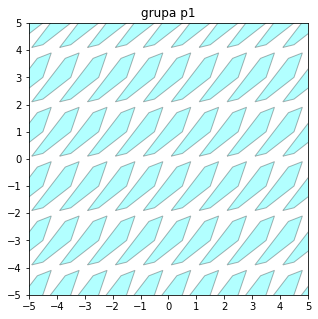
\includegraphics[width=\textwidth]{output_87_1.png}
    \label{fig:f10}
  \end{subfigure}
  \begin{subfigure}[b]{0.22\textwidth}
    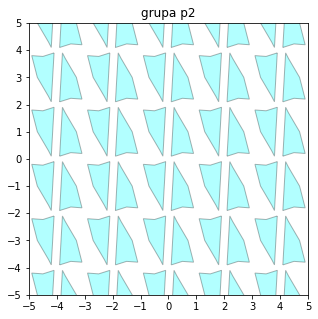
\includegraphics[width=\textwidth]{output_87_2.png}
    \label{fig:f11}
  \end{subfigure}
  \begin{subfigure}[b]{0.22\textwidth}
    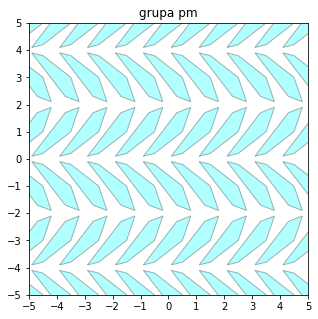
\includegraphics[width=\textwidth]{output_87_3.png}
    \label{fig:f12}
   \end{subfigure} 
   \begin{subfigure}[b]{0.22\textwidth}
    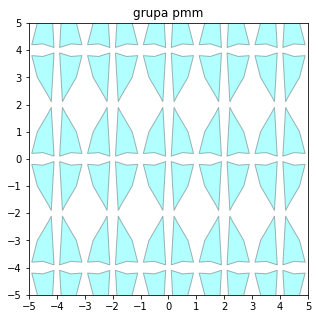
\includegraphics[width=\textwidth]{output_87_4.png}
    \label{fig:f13}
  \end{subfigure}
\end{figure}

\begin{figure}[H]
  \begin{subfigure}[b]{0.22\textwidth}
    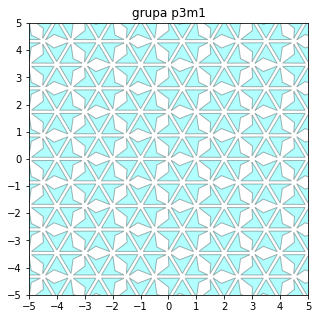
\includegraphics[width=\textwidth]{output_87_6.png}
    \label{fig:f14}
  \end{subfigure}
  \begin{subfigure}[b]{0.22\textwidth}
    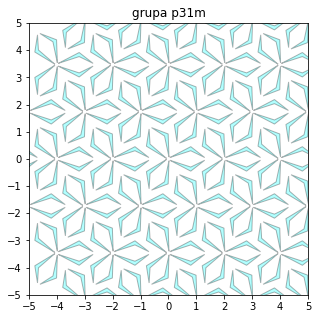
\includegraphics[width=\textwidth]{output_87_7.png}
    \label{fig:f15}
  \end{subfigure}
  \begin{subfigure}[b]{0.22\textwidth}
    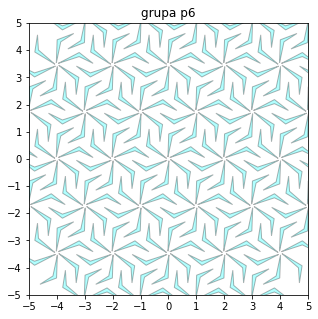
\includegraphics[width=\textwidth]{output_87_8.png}
    \label{fig:f16}
    \end{subfigure}
   \begin{subfigure}[b]{0.22\textwidth}
    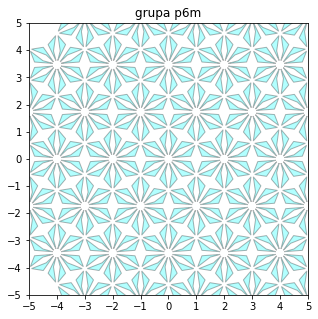
\includegraphics[width=\textwidth]{output_87_9.png}
    \label{fig:f17}
  \end{subfigure}
\end{figure}


   % \begin{center}\rule{0.5\linewidth}{\linethickness}\end{center}

    \section{Konstrukcija fundamentalne oblasti}\label{dirihleova-fundamentalna-oblast} Kada je data kristalografska grupa postavlja se pitanje kako mo\v zemo konstruisati fundamentalne poligone za tu grupu. U ovom poglavlju \' cemo opisati Dirihleov domen kao i uop\v stenja Dirihleovog domena.
\subsection{Voronojev dijagram}


Posmatrajmo ravan $\pi$ i dve proizvoljne ta\v cke $A$ i $B$ u njoj. Podelimo je simetralom du\v zi $AB$ na dve poluravni $\pi _A$ i $\pi _B$, tako da $A \in \pi _ A$ i $B \in \pi _B$. Jasno je da su sve ta\v cke na simetrali jednako udaljene od ta\v caka $A$ i $B$, kao i da je svakoj ta\v cki u $\pi _A$ bli\v za ta\v cka $A$ nego ta\v cka $B$ i obrnuto. 
Na taj na\v cin smo sve ta\v cke ravni $\pi$ podelili na dva podskupa prema tome kojoj od ta\v caka $A$ i $B$ su bli\v ze, a na rubu tih skupova (simetrala du\v zi $AB$) su ta\v cke koje su jednako udaljene od $A$ i $B$.

Uop\v stimo ovaj postupak za kona\v can broj po\v cetnih ta\v caka.

Ozna\v cimo redom sa $\pi _{XY}$ i $\pi _{YX}$ otvorene poluravni kojima simetrala du\v zi $XY$ deli ravan $\pi$ na dve poluravni tako da $X \in \pi _ {XY}$ i $Y \in \pi _{YX}$. 

Ukoliko na po\v cetku imamo tri ta\v cke $A$, $B$ i $C$, tada je $\pi _{AB}$ skup svih ta\v caka u ravni kojima je ta\v cka $A$ bli\v za nego ta\v cka $B$ i $\pi _{AC}$ skup ta\v caka kojima je ta\v cka $A$ bli\v za nego ta\v cka $C$, pa je $\pi _{AB} \cap \pi _{AC}$ skup ta\v caka kojima je ta\v cka $A$ najbli\v za ta\v cka.

Primenom ovog postupka na  $n$ ta\v caka, $A_1$, $A_2$, ... $A_n$ dobijamo da je skup ta\v caka kojima je $A_i$ najbli\v za  jednak $$\bigcap _{1\leq j\leq n,\; j\neq i} \pi_{A_i A_j}$$

Ovakvku podelu ravni na oblasti prema rastojnju od datih ta\v caka naziva se \emph{Voronojevim dijagramom} prema ruskom mateti\v caru \emph{Georgiju Voronoju}.

\begin{definition}%(voronijev dijagram)
Za skup ta\v caka $S$ u ravni, Voronojev dijagram predstavlja podelu ravni na zatvorene disjunktne oblasti $V_S(A_i)$, koje nazivamo Voronojevim \' celijama, tako da
$$ (\forall X \in V_{S}(A))(\forall B \in S\setminus \{A\})\quad d(X,A)\leq d(X,B) $$
$$ \bigcup_{\forall A \in S} V_{S}(A) = \mathbb{E}^2 $$

\end{definition}

Iz prethodnog razmatranja proizilazi da je
$$V_S(A) = \bigcap _{B \in S \setminus \{A\}} \pi_{AB}$$

\subsection{Dirihleov domen}

Voronojevi dijagrami daju jedan metod konstruisanja fundamentalnog domena kristalografske grupe $G$ tako \v sto za skup $S$ uzmemo orbitu neke ta\v cke $X$. Tada Voronojev dijagram predstavlja poplo\v cavanje ravni pod dejstvom grupe $G$, a svaka \' celija dijagrama je fundamentalna oblast. \\
Takav fundamentalni domen naziva se \emph{Dirihleov domen}.

Ozna\v cimo sa $O_G(X)$ orbitu ta\v cke $X$,  \v sto zna\v ci 
$$O_G(X) = \{g(X)\:|\:g \in G\} $$

\begin{definition}
Za datu ta\v cku $X$ i kristalografsku grupu $G$ Dirihleov domen se defini\v se kao  
$$D_G(X) = \{Y \in \mathbb{E}^2\:|\:(\:\forall g \in G \setminus \{I\})\:(d(Y,X)\leq d(Y,g(X))\:\}$$
\end{definition}

\noindent Doka\v zimo da ovako definisan Dirihleov domen predstavlja fundamentalni poligon.
Dirihleov domen mo\v zemo posmatrati kao \' celiju Voronojevog dijagrama 
$$D_G(X)= V_{O_G(X)}(X)$$

\noindent Kako va\v zi $d(g(X), g(Y))= d(X,Y)$ to je $D_G(g(X)) = g(D_G(X))$  
Tako\dj e primetimo da $$Y \in  O_G(X) \implies O_G(Y) = O_G(X) $$
Na osnovu prethodnog zaklju\v cujemo da va\v zi

$$\bigcup_{g\in G}g(D_G(X)) = \bigcup_{g\in G}D_G(g(X)) = \bigcup_{y \in O_G(X)}D_G(Y)
= \bigcup_{Y \in O_G(X)}V_{O_G(Y)}(Y) = \mathbb{E}^2$$

\noindent Time smo dokazali prvi uslov iz definicije fundamentalnog poligona, da slike poligona pokrivaju celu ravan.

\noindent Sli\v cno zaklju\v cujemo da za $Y = g(X)$
$$g(D_G(X)) = D_G(Y) = V_{O_G(Y)}(Y)$$ \v sto zna\v ci da su $D_G(X)$ i $D_G(Y)$ razli\v cite \' celije Voronojevog dijagrama, pa im unutra\v snjosti nemaju preseka. 

Time smo dokazali i drugi uslov iz definicije fundamentalnog poligona, da se slike poligona ne preklapaju. Dakle, dokazali smo da je $D_G(X)$ fundamentalni domen grupe $G$.

Na narednim slikama su prikazani primeri Dirihleovog domena za grupu \textbf{p6} i prozvoljne ta\v cke. 
Grupa \textbf{p6} je generisana rotacijama za ugao \(\frac{2\pi}{3}\) oko jednog
i \(\frac{\pi}{3}\) oko ostala dva temena trougla sa uglovima \(\frac{2\pi}{3}\), \(\frac{\pi}{6}\) i \(\frac{\pi}{6}\).



  \begin{figure}[H]
  \begin{subfigure}[b]{0.3\textwidth}
    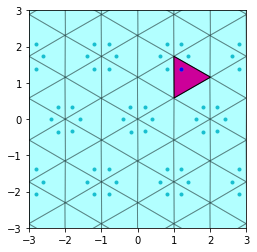
\includegraphics[width=\textwidth]{output_10_0.png}
    \label{fig:f1}
  \end{subfigure}
  \begin{subfigure}[b]{0.3\textwidth}
    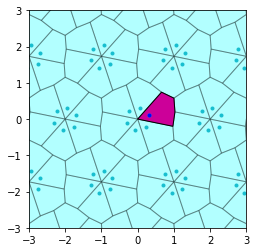
\includegraphics[width=\textwidth]{output_13_0.png}
    \label{fig:f2}
  \end{subfigure}
  \begin{subfigure}[b]{0.3\textwidth}
    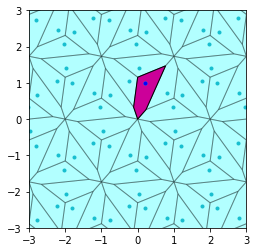
\includegraphics[width=\textwidth]{output_12_0.png}
    \label{fig:f3}
  \end{subfigure}
\end{figure}


    \subsection{Uop\v sten Dirihleov domen za vi\v se ta\v caka}\label{konstrukcija-dirihleove-fundamentalne-oblasti}
    
Sli\v cno Dirihleovom domenu za jednu ta\v cku,  mo\v zemo posmatrati domen generisan dvema ta\v ckama. Tada nam je $O_G(\{X,Y\})$ skup ta\v caka koje se mogu dobiti izometrijama od jedne od te dve ta\v cke. Posmatrajmo Voronojev dijagram nad svim ta\v ckama orbite $O_G(\{X,Y\})$. Unija Voronojevih \' celija za ta\v cku $X$ i za ta\v cku $Y$ predstavlja fundamentalni domen grupe $G$, \v sto je u op\v stem slu\v caju iskazano narednim tvr\dj enjem.
\begin{tvrdjenje}
Ako je dat kona\v can skup ta\v caka $S$ ravni na koju deluje kristalografska grupa $G$, tada je 
$$D_G(S) = \{x \in \mathbb{E}^2\:|\:(\:\forall g \in G \setminus \{I\})\:(d(X,S)\leq d(X,g(S))\:\}$$

fundamentalni domen grupe $G$, gde je $d(X,S) = \min_{Y \in S} d(X,Y)$ i va\v zi 
$$D_G(S) = \bigcup_{X \in S} V_{O_G(S)}(X) $$ 
\end{tvrdjenje}

%Doka\v zimo prvo drugi deo tvr\dj enja. 
%Posmatrajmu ta\v cku $Y$ takvu da $Y \in D_G(X)$. Tada je $(\:\forall X_1 \in O_G(S))\:(d(Y,X)\leq d(Y,X_1)$
%$$D_G(S) = \bigcup_{X \in S} D_G(X) $$

%nastavice se

\begin{samepage}
Na primerima vidimo uop\v steni Dirihleov domen za dve, tri i \v cetiri proizvolje ta\v cke i grupu \textbf{p6}.

\begin{figure}[H]
  \begin{subfigure}[b]{0.3\textwidth}
    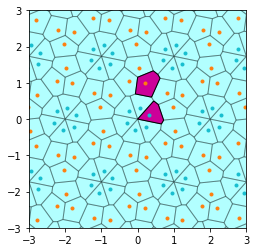
\includegraphics[width=\textwidth]{output_14_0.png}
    \label{fig:f4}
  \end{subfigure}
  \begin{subfigure}[b]{0.3\textwidth}
    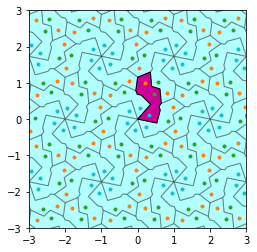
\includegraphics[width=\textwidth]{output_15_0.png}
    \label{fig:f5}
  \end{subfigure}
  \begin{subfigure}[b]{0.3\textwidth}
    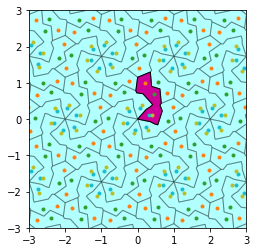
\includegraphics[width=\textwidth]{output_16_0.png}
    \label{fig:f6}
  \end{subfigure}
\end{figure}
\end{samepage}

    \subsection{Uop\v steni Dirihleov domen za poligon}\label{modifikacija-fundamentalne-oblasti-na-osnovu-podfundamentalne}
Definicija Dirihleovog domena se mo\v ze uop\v stiti i kada skup $S$ nije kona\v can, a konstrukcija pomo\' cu Voronojevog dijagrama u tom slu\v caju se mo\v ze izvesti kao grani\v cna vrednost kada biramo sve ve\'ci broj ta\v caka.

Neka je dat poligon $P$ tako da se slike poligona u orbiti ne presecaju. 

Neka je $S_0$ skup temena poligona $P$, a $S_n$ skup u kome su pored temena poligona i po $n$ ta\v caka sa svake od stranica poligona na jednakim rastojanjima u okviru stranice.

Na slici 7 je dat primer za $D_G(S_0)$.On jeste fundamentalni domen ali primetimo da ne obuhvata ceo poligon $P$.

Na slici 8 je prikazan $D_G(S_1)$, gde su uklju\v cena i sredi\v sta stranica i primeti\' cujemo da taj fundamentalni domen bolje pokriva po\v cetni poligon. 


Uop\v steni Dirihleov domen za poligon mo\v zemo da defini\v semo isto kao i za kona\v can skup
$$D_G(P) = \{X \in \mathbb{E}^2\:|\:(\:\forall g \in G \setminus \{I\})\:(d(X,P)\leq d(X,g(P))\:\}$$
pri \v cemu je $d(X,P) = \inf_{Y \in P} d(X,Y)$ i tada va\v zi
$$ D_G(P) = \lim _{n\to \infty} D_G(S_n) $$


Za prakti\v cne potrebe mo\v zemo gledati dovoljno veliko $n$. Na slici 9 je dat primer za $D_G(S_{50})$

  \begin{figure}[H]
  \begin{subfigure}[b]{0.3\textwidth}
    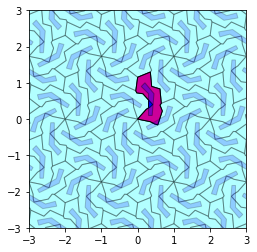
\includegraphics[width=\textwidth]{output_17_0.png}
    \label{fig:f7}
  \end{subfigure}
  \begin{subfigure}[b]{0.3\textwidth}
    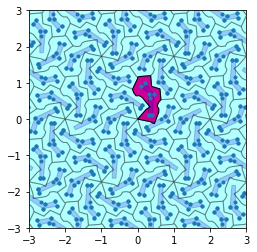
\includegraphics[width=\textwidth]{output_18_0.png}
    \label{fig:f8}
  \end{subfigure}
  \begin{subfigure}[b]{0.3\textwidth}
    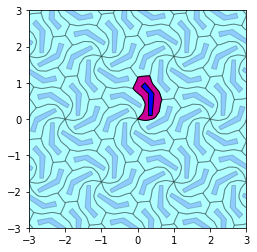
\includegraphics[width=\textwidth]{output_21_2.png}
    \label{fig:f9}
  \end{subfigure}
\end{figure}

\begin{samepage}
 Na slede\' cim slikama su dati primeri uop\v stenih dirihleovih domena za isti poligon u raznim kristalografskim grupama.
 \begin{figure}[H]

  \begin{subfigure}[b]{0.3\textwidth}
    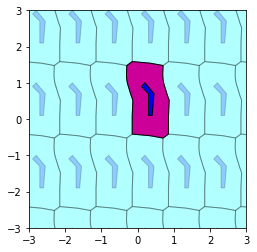
\includegraphics[width=\textwidth]{output_21_1.png}
    \label{fig:f20}
    \caption{grupa \textbf{p1}}
  \end{subfigure}
  \begin{subfigure}[b]{0.3\textwidth}
    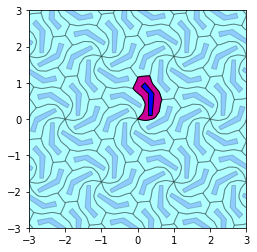
\includegraphics[width=\textwidth]{output_21_2.png}
    \label{fig:f21}
    \caption{grupa \textbf{p2}}
  \end{subfigure}
  \begin{subfigure}[b]{0.3\textwidth}
    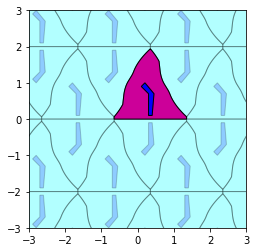
\includegraphics[width=\textwidth]{output_21_10.png}
    \label{fig:f24}
    \caption{grupa \textbf{pg}}
  \end{subfigure}

  \begin{subfigure}[b]{0.3\textwidth}
    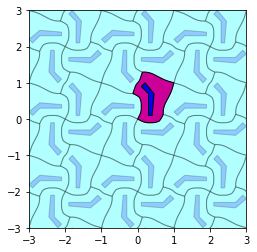
\includegraphics[width=\textwidth]{output_21_4.png}
    \label{fig:f23}
    \caption{grupa \textbf{p4}}
  \end{subfigure}
  \begin{subfigure}[b]{0.3\textwidth}
    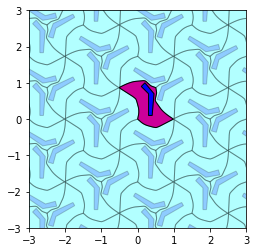
\includegraphics[width=\textwidth]{output_21_3.png}
    \label{fig:f22}
    \caption{grupa \textbf{p3}}
  
  \end{subfigure}
  \begin{subfigure}[b]{0.3\textwidth}
    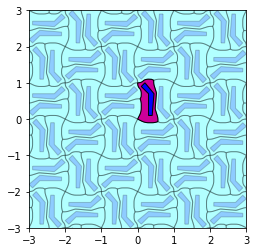
\includegraphics[width=\textwidth]{output_21_7.png}
    \label{fig:f25}
    \caption{grupa \textbf{cmm}}
  \end{subfigure}
\end{figure}
\end{samepage}

\quad \\ \qquad
    \section{Implementacija}\label{implementacija}

    Na osnovu prethodno opisanih metoda konstrukcije fundamentalnih domena implementirana je ra\v cunarska implementacija koja omogu\' cava interaktivnu konstruktciju fundamentalnog domena za izabranu kristalografsku grupu.
Aplikacija se mo\v ze koristiti za dizajniranje zanimljivih poplo\v cavanja.
Implementirana je u programskom jeziku Python.

Na prikazanim izgledima ekrana korisnik dodavaje ta\v cku po ta\v cku putem klika na mi\v su i na taj na\v cin oblikovuje fundamentalnu oblast. Za konstrukciju fundamentalnih domena pored izabranih ta\v caka kori\v s\' cene su dodatne ta\v cke izme\dj u njih kako bi oblik fundamentalnog domena bio "mek\v si". 


\begin{figure}[H]

  \begin{subfigure}[b]{0.33\textwidth}
    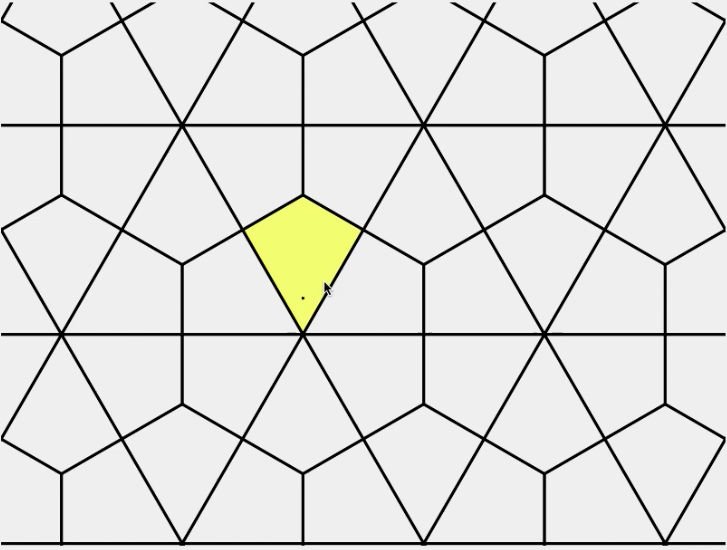
\includegraphics[width=0.9\textwidth]{sl1.png}

  \end{subfigure}
  \begin{subfigure}[b]{0.33\textwidth}
    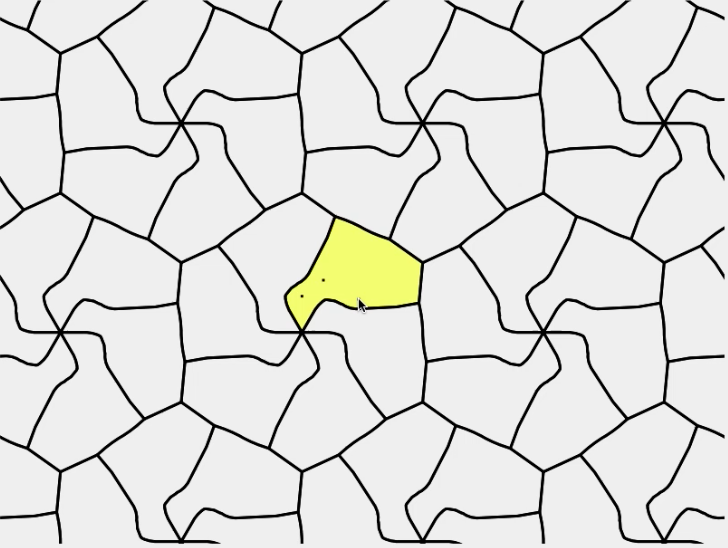
\includegraphics[width=0.9\textwidth]{sl2.png}

  \end{subfigure}
  \begin{subfigure}[b]{0.33\textwidth}
    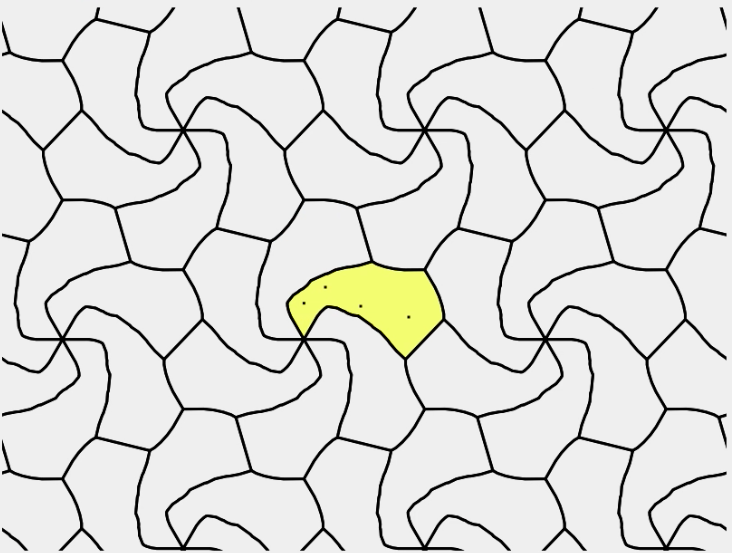
\includegraphics[width=0.9\textwidth]{sl6.png}

  \end{subfigure}

\quad

  \begin{subfigure}[b]{0.33\textwidth}
    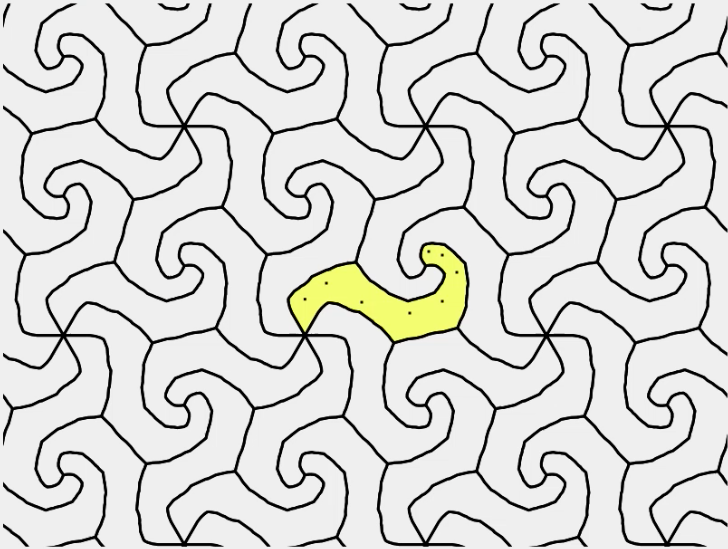
\includegraphics[width=.9\textwidth]{sl3.png}

  \end{subfigure}
  \begin{subfigure}[b]{0.33\textwidth}
    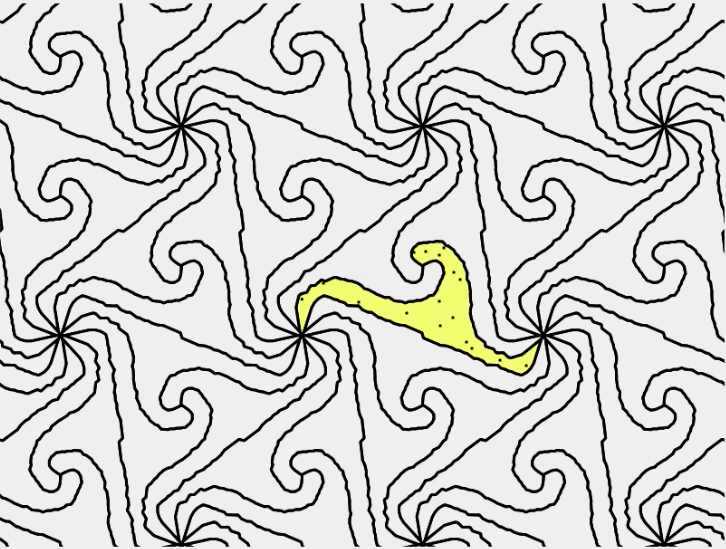
\includegraphics[width=.9\textwidth]{sl4.png}

  
  \end{subfigure}
  \begin{subfigure}[b]{0.33\textwidth}
    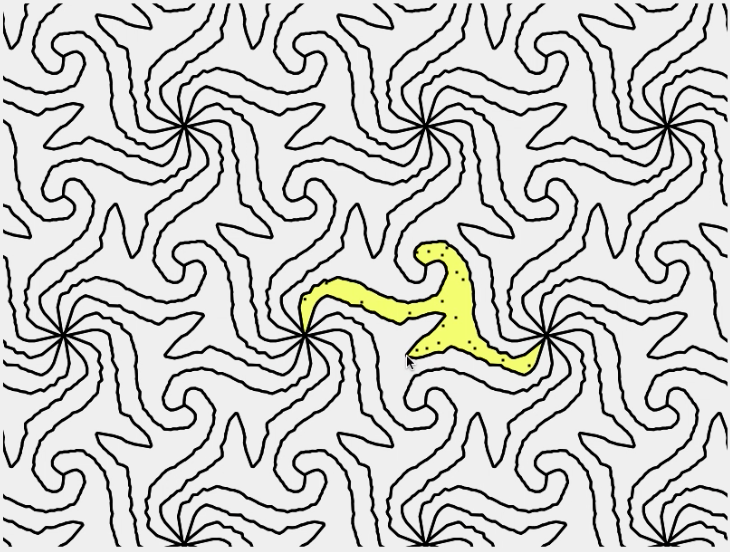
\includegraphics[width=.9\textwidth]{sl5.png}

  \end{subfigure}
  
\end{figure}


\begin{thebibliography}{99}
\bibitem{1}  Carne, T. K. "Geometry and groups." Lecture notes, Cambridge University (2006). 
 \bibitem{4}  Kaplan, Craig S. "Introductory tiling theory for computer graphics."{} Synthesis Lectures on Computer Graphics and Animation 4.1 (2009): 1-113. 
 \bibitem{6}  Kilgore, J. "Fundamental Domains of Discrete Groups Acting on Euclidean Space." (2012). 
 \bibitem{2} Lučić, Z., and Molnár, E. "{}Combinatorial classification of fundamental domains of finite area for planar discontinuous isometry groups." Archiv der Mathematik 54.5 (1990): 511-520.
\bibitem{1} Molnár, E. "Nice tiling, nice geometry." Teaching Mathematics and Computer Science, Debrecen (2012): 269-280.


\bibitem{5} 
  Schattschneider, D. "The plane symmetry groups: their recognition
  and notation." \emph{The American Mathematical Monthly} 85.6 (1978):
  439-450.


\end{thebibliography}

    % Add a bibliography block to the postdoc
    
    
    
    \end{document}
